% Literature Review
% 01/03/11
% (Use \include{filename} in diss proposal file

\documentclass[a4paper,12pt]{report} 	% report used for dissertations

\usepackage{anysize} 		% allows me to set margins
\usepackage{indentfirst}
\usepackage{apacite}		% for apa style
\usepackage{graphicx}		% for graphics

\marginsize{1.5in}{1.5in}{1.25in}{1.25in}	% left, right, top, bottom
\linespread{2}			% double-spacing
\begin{document}

\pagenumbering{roman}

\setcounter{page}{2}

\listoftables
\listoffigures
\newpage
\pagenumbering{arabic}


\begin{flushleft}			% generates left-aligned paragraphs
\setlength{\parindent}{30pt}	% This starts every paragraph with an indent

\begin{center}
EVOLVING SYNTHESIS ALGORITHMS USING A MEASURE OF LOCAL TIMBRE SIMILARITY
\end{center}

						
\section*{\centering CHAPTER I \\RESEARCH OBJECTIVE}
\subsection*{Statement of Problem}
Timbre has played an increasingly important role in composition since the beginning of the 20th century. With the advent of digital technology, composers have been given the power to generate sounds with boundless timbral variation. However, true timbral exploration is still out of reach for all but the the most technically inclined and dedicated, as the mechanisms that provide timbre control (synthesis algorithms) are often unintuitive unless one has a strong understanding of the mathematics that underly their sound production; and even in this case, achieving a specific desired timbre often requires a large amount of trial-and-error. To further complicate things, a variety of synthesis algorithms exist, each suited to only produce a subset of all possible timbre. Therefore, in order to successfully generate a desired timbre (or explore a specific region of timbre space) one must first choose an appropriate synthesis algorithm and then find an appropriate parameter set for the chosen topology. Placing this burden on the composer requires them to spend more time on trial-and-error searching and less time composing. The less technically inclined the composer is, the more time they will probably spend performing tasks that are not beneficial to their compositional process. It is our goal to shorten this search process for all composers, which we hope will also remove the inherent bias towards the mathematically sophisticated.
	
Approaching timbre matching through the lens of automatic programming, we will develop a system intended to automate this search process by automatically generating a synthesis topology well suited to the desired timbre, while simultaneously finding an appropriate parameter set that realizes it. This system will perform an intelligently directed search through all possible synthesis topologies and parameter sets in order to find a suitable algorithm to produce the desired timbre (which will be supplied by the user).

\subsection*{Statement of Subproblems}
\begin{enumerate}
\item To determine an appropriate environment to automatically generate synthesis topologies within and to establish an acceptable input-space representation for such topologies.
\item To decide upon a well-suited intelligent search algorithm for navigating the input space defined by subproblem 1 and to find the best architecture for that algorithm.
\item To find ways of restricting the search space and making the search algorithm more efficient and powerful without omitting optimal solutions.
\item To develop an objective timbre space in which distances are semantically meaningful, information regarding the temporal evolution of timbre is retained, and whose elements are invariant to changes in pitch and loudness.
\item To determine an appropriate similarity metric in the objective timbre space found in subproblem 4 that will be appropriate for comparing time-varying timbral content. This metric will help define an objective landscape over the synthesis algorithm input space whose global maximum (or minimum) will correspond to the desired solution.
\item To combine the solutions of subproblems 1-5 into a system implementation capable of automatically generating synthesis algorithms that not only match the target input, but that also exhibit attractive properties for any synthesis algorithm.
\end{enumerate}

\subsection*{Definitions}
\begin{description}
\item[Synthesis (Input) Space] - The set containing all possible combinations of atomic code blocks and parameters which can be used to build synthesis algorithms.
\item[Synthesis Topology] - A specific combination of atomic code blocks that produces audio. This will include algorithms that take basic waveforms (e.g. sine, square wave, sawtooth, impulse train, white noise, etc) as input as well as those that take more complex input (e.g. recorded audio). A single topology can represent a different point in synthesis space for every unique parameter set that can be assigned to it. 
\item[Timbre (Output) Space] - The set containing all possible timbres and a corresponding distance metric defined on that set, which represents semantic timbre similarity.
\item[Automatic programming] - `A systematic method for getting computers to automatically solve a problem starting from a high-level statement of what needs to be done' (Vanneschi, 2004, p. 10). 
\item[Intelligent Search Algorithm] - An algorithm that relies on assumptions about the search space in order to develop ways of leading the search towards optimal regions of that space faster than a random exhaustive search would.
\item[Local timbre representation] - A mathematical representation of the timbre percept over a short period of time (as opposed to �global� timbre similarity). Local timbre also differs from short-time timbre, in that the latter is used in the literature to refer to a timbre representation specifically on the order of a spectral analysis frame.
\item[Objective landscape] - This defines a mapping between points in the input space and how well they achieve their stated goal.

\end{description}

\subsection*{Need for Study}

The proposed research will attempt to develop a system that, given a desired location timbre space, is able to construct a synthesis algorithm with a low-dimensional parameter set, low time-complexity, and low space-complexity that maps to that location. By intelligently choosing which algorithm and parameter mapping to use for a given region of timbre space, this system will act as a meta-synthesizer able to automatically construct efficient synthesis topologies for any timbral region.

This research has the potential to impact a number of areas of study including computer music, music information retrieval, artificial intelligence (of which automatic programming research is a subset), and signal processing.

Practically speaking, the proposed system would extend the sonic palette of any composer (or producer) utilizing digital audio effects or synthesis algorithms regularly in their works. The availability of a larger timbral tool set for composers would naturally lead to more experimentation and timbral exploration as composers would be able to create with timbre in ways previously not available to them. Placing the burden of timbral search on the computer would also free up more time to compose, likely leading to increased compositional output; a benefit to the music community as a whole.

In constructing this system, we will investigate more appropriate ways of measuring local timbre similarity. Local timbral similarity is a far less researched topic than global timbral similarity in the MIR community. However, we believe that much can be learned about timbre on a local time scale, especially in cases where its specific temporal evolution contributes greatly to its perception. Also, by investigating new objective timbre spaces whose distance measurements are semantically meaningful, this research will benefit MIR researchers interested in, for example, instrument classification, song similarity, audio fingerprinting, and vocalist recognition.

This study would also contribute to the growing body of research targeted toward the use of artificial intelligence in artistic applications. Most research in this area deals with the creation of artistic works by machines and there is much less work focused on using artificial intelligence to generate new tools for human creators interested in a more traditional creation process. This research hopes to change that trend by exemplifying the importance of tool generation for artists that are not satisfied with their present means of creation.

Specifically, within the domain of artificial intelligence, almost all practical automatic programming research targets designing software for solving scientific problems (e.g. robot mechanics, circuit board design). Therefore, this study, drawing primarily from the automatic programming research community, will integrate a domain typically interested in solving scientific problems with one of artistic creation in a way not yet approached rigorously.

Therefore, this study is significant from both theoretical and practical perspectives and will contribute to a number of different disciplines ranging from applied computer science and digital signal processing to computer music composition, music production, and music information retrieval.

\newpage
\section*{\centering CHAPTER II\\ RELATED LITERATURE} 	% * suppresses heading numbers
\subsection*{Sound Synthesis}
Timbre is a fundamental parameter of music, yet total and precise timbre control cannot be realized - or, at the very least, is severely limited - by acoustic means. Even the most skilled players are constrained by the physics of their instruments' sound production mechanisms (Wessel \& Wright, 2002, p. 11). However, with the advent of digital technology, the sound generator can be separated from its control interface and therefore no longer reliant on its physical properties (Malloch, Birnbaum, Sinyor, \& Wanderley, 2006, p. 1).  The resulting timbral freedom introduced by digital music instruments could not have come at a better time as Western compositional practice saw timbre taking on an increasingly important role soon after the turn of the twentieth-century (Klingbeil, 2009, p. 1). In investigating the increasingly common compositional use of timbre, Nicola Bernardini and J�ran Rudi (2001) write that by providing a `different, deeper and total control over timbre [computer music composition has placed a] stronger focus on the timbral aspects of composition -- on the micro-level.' (p. 3). This increased focus has been responsible for the design of numerous sound synthesis algorithms over the past fifty years, each successful at providing the composer with the means to produce and effectively manipulate desired timbres to varying degrees of success.

The different approaches used in designing synthesis algorithms have varied widely throughout the history of sound synthesis. While there are a number of sources (e.g. (Roads, 1996), (Miranda, 1998), (Cook, 2002)) that attempt to outline all of these methods, Miller Puckette�s \emph{The Theory and Technique of Electronic Music} (2007) is the most relevant to our research in that it provides a complete summary of the various approaches towards sound synthesis design in the context of PD (Pure Data), an open-source graphical programming language written by Puckette that is almost identical to Max (also written by Puckette). This book in combination with Puckette�s earlier paper, \emph{Combining Event and Signal Processing in the MAX Graphical Programming Environment} (1991), provides a comprehensive look into designing synthesis algorithms using a graphical programming environment. The intent of these writings is not to compare and contrast the efficacy of the algorithms presented, but instead only to illustrate their inner workings. However, when a composer is ready to select a specific synthesis algorithm to work with, the results of such comparisons are paramount to the decision-making process. In order to assess the strengths and weaknesses of each algorithm, one must have a clear understanding of the desirable properties of a timbre producer/manipulator.

These properties have been discussed by a number of important people in the field of computer music at various levels of depth (e.g. (Smith, 1991), (Jaffe, 1995), (Wessel \& Wright, 2002)). Smith's treatment is relatively superficial in large part because these properties are not his paper's main focus. Jaffe's list of properties presume that a synth's main purpose is to mimic a real-world sound producing body, which is not always necessarily the case. Wessel and Wright mix the desirable properties of synthesis algorithms with those of control interfaces, often blurring the lines between the two within the same listed property. More recently, in his treatment of composing with timbre, Nicol (2005, p. 40) provides four desirable properties of an ideal synthesizer: `fast synthesis' (i.e. computational efficiency), a `wide timbral range' (i.e. the ability to produce any desirable timbre), `easy parameterization' (i.e. an intuitive, low-dimensional mapping between parameters and sound), and `low data requirements' (i.e. low memory storage requirements). In other words, an ideal synthesizer will provide the composer with an intuitive, low-dimensional parameter set that they may use to achieve (and manipulate) any desired timbre. Additionally, the underlying synthesis algorithm will ideally work in real-time and use a small amount of memory.

One of the most comprehensive comparative studies of synthesis algorithms is presented by Tolonen, V\aa lim\aa ki, and Karjalainen (1998). In this report, the authors categorize each synthesis algorithm under evaluation into one of four groups: abstract algorithms, sampling and processed recordings, spectral methods, and physical models (as originally proposed in (Smith, 1991)). Among the many algorithms treated, Tolonen, V\aa lim\aa ki, and Karjalainen choose the most popular (also known as `classical' synthesis algorithms) to evaluate and find that their variants within each category perform similarly in regards to the proposed criteria (1998, p. 101). The classical synthesis methods investigated in their study were sampling synthesis (sampling and processed recordings), granular synthesis (sampling and processed recordings), additive synthesis (spectral methods), subtractive synthesis (spectral methods), FM synthesis (abstract algorithms), and digital waveguide synthesis (physical models).

Sampling synthesis `is a method in which recordings of relatively short sounds are played back.' (Tolonen, V\aa lim\aa ki, \& Karjalainen, 1998, p.10). Using sampling, one can turn any audio recording into a musical instrument by simply assigning the playback of the recording to a switch (Heise, Hlatky, \& Loviscach, 2009, p.1). This type of synthesis dates back to the 1920's and certainly became prominent in 1950 when Pierre Schaeffer founded the Studio de Musique Concrete in Paris (Tolonen, V\aa lim\aa ki, \& Karjalainen, 1998, p. 3). Like all sampling and processed recordings methods, sampling synthesis� flexibility is dependent on the size of the database containing the pre-recorded audio segments. Thus, to obtain a truly flexible sampling synthesizer `the required amount of memory storage is huge' (Tolonen, V\aa lim\aa ki, \& Karjalainen, 1998, p. 11). As the flexibility of the system grows and one has enough material to generate small variations in timbre, doing so becomes more difficult as the number of samples to choose from during any single discrete movement in timbre space becomes unweildy. Thus, while sampling synthesis is computationally efficient and requires a low-dimensional parameter set, there is a fundamental tradeoff between its ability to generate a wide variety of timbral material and the amount of memory it requires. It is also nontrivial to transform a given timbre in a smooth way, which, in his more recent survey of synthesis techniques, Smith writes is the true `fundamental problem with sampling synthesis' (2006, p. 22).

Granular synthesis `is a set of techniques that share a common paradigm of representing sound signals by ``sound atoms'' or grains...the synthetic sound signal is composed by adding these elementary units in the time domain' (Tolonen, V\aa lim\aa ki, \& Karjalainen, 1998, p.13). In his dissertation on analysis/synthesis techniques (which we be covered later), Klingbeil adds that 'granular synthesis may be viewed as a particular specialization of sampling synthesis...[It] offers the possibility to decouple the time and frequency evolution of a sound, as well as impart particular characteristics modulating between rough, smooth, or stochastic textures' (2009, p. 6). Thus, unlike sampling synthesis, granular synthesis allows one to transform smoothly between timbres. However, this comes at the price of a higher dimensional parameter space, forcing the user to specify `the shape of the overall ``cloud'', the fundamental frequency, the way in which the individual grains are generated, the structure of the individual grains used, etc' (Johnson, 1998, p. 5). In Nicol's dissertation investigating mappings between synthesis parameter spaces and timbre spaces, he notes that the non-intuitive mapping between this high dimensional parameter space and timbre space makes `emulation of target timbres a non-trivial process' (Nicol, 2005, p. 49). Granular synthesis requires less memory than sampling synthesis, but is also less efficient (although real-time algorithms do exist). Vercoe, Gardner, and Scheirer point out that granular synthesis is `best suited to the generation of noisy or textural sounds like water, wind, applause, and fire' (1998, p. 6).

Additive synthesis `is a method in which a composite waveform is formed by summing sinusoidal components to produce a sound' (Tolonen, V\aa lim\aa ki, \& Karjalainen, 1998, p. 17). Based on Fourier analysis, `additive synthesis can in theory synthesize arbitrary sounds if an unlimited number of oscillators is available' (Tolonen, V\aa lim\aa ki, \& Karjalainen, 1998, p. 94). However, as the numbers of oscillators increase, the number of controllable parameters increase and therefore what adding oscillators gains in flexibility, it loses in controllability (Klingbeil, 2009, p. 7). It is because of this that additive synthesis is best utilized for generating harmonic or almost harmonic signals where little noise is present (Vercoe, Gardner, \& Scheirer, 1998, p. 5). Additive synthesis also requires a number of parameters to be changed simultaneously in order to move even a small distance in timbre space, which is unattractive. The desirable properties that additive synthesis satisfies are low storage (although the control data can require a lot of memory) and the ability to generate, in theory, any timbre, but it can be computationally expensive depending on the number of oscillators used and its parameter space is high-dimensional and therefore difficult to control.

Subtractive synthesis is similarly based on Fourier analysis, but works by subtracting sinusoids from a spectrally rich source to generate material rather than building up material by adding sinusoids together, as in additive synthesis. The `subtraction' is performed by a time-varying filter whose coefficients are supplied by the user. In order to achieve complex and temporally evolving sounds, the parameter space can grow to the size of additive synthesis and therefore will suffer from the same controllability issues (Tolonen, V\aa lim\aa ki, \& Karjalainen, 1998, p. 48). If one uses a simple network of filters to try to reduce the size of the parameter space, `the resulting tones have a distinctive ``analog synthesizer'' character that, while sometimes desirable, is difficult to avoid' (Vercoe, Gardner, \& Scheirer, 1998, p. 5). Thus, one must trade timbral flexibility with the controllability of the algorithm. Similar to additive synthesis, the control data can require a lot of memory during sound production. Also, the efficiency of the algorithm and the facility to move around timbre space varies with the complexity of the time-varying filter or network of filters.

FM synthesis, in its most basic form, contains two oscillators, which are connected so that one oscillator�s waveform modulates the frequency of the other. There are only a few parameters with which to generate a large range of timbral material, which is desireable, but due to an inherent nonlinear mapping between parameter space and control space, `FM has become widely regarded as a difficult synthesis type to control' (Mitchell \& Creasey, 2007). This is for two reasons. First, the nonlinearity provides a non-intuitive relationship between a given set of parameters and the sound it produces (Nicol, 2005, p. 45). Second, a  nonlinear mapping means that small changes in the input parameters can map to large changes in the timbre and so fine timbral manipulation can be difficult (Jaffe, 1995, p. 2). Another undesirable quality of FM synthesis is that the characteristic FM sound is `fairly metallic, so the FM output is often filtered in order to produce a more natural sound' (Nicol, 2005, p. 45). The benefits of FM synthesis are that is `is very cheap to implement, uses little memory, and [as previously mentioned] the control stream is sparse' (Tolonen, V\aa lim\aa ki, \& Karjalainen, 1998, p. 92).

Digital waveguides are `based on a general solution of the wave equation in a one-dimensional homogeneous medium' (Tolonen, V\aa lim\aa ki, \& Karjalainen, 1998, p. 63). They are basic linear time-invariant (LTI) structures that allow one to develop physical models of various instruments. When digital waveguides are used to synthesize sounds based on physical models of sound-generating objects, their parameters are intuitive and small in number, aiding in timbral manipulation. However, any one waveguide network will only be able to generate a small subset of timbres within timbre space and therefore will not be flexible in the way that, for example, additive synthesis is. Also, as Smith (1992) comments in his seminal paper on digital waveguides `new models must be developed for each new kind of instrument, and for many instruments, no sufficiently concise algorithm is known' (p. 86). In fact, as Tolonen, V\aa lim\aa ki, and Karjalainen point out, any sound producing object that requires a two- or three-dimensional waveguide mesh to represent its governing physics will be computationally expensive to model and therefore only simple physical models based on waveguides will be able to run in real-time (1998, p. 99-100). Thus, digital waveguides provide a low-dimensional, intuitive parameter set and low storage requirements, but can be computationally expensive for complex sounds and require separate topologies for each region of timbre space (Nicol, 2005, p. 50).

A comparative study of various sound synthesis techniques, such as that carried out by Tolonen, V\aa lim\aa ki, and Karjalainen elucidates the strengths and weaknesses of each algorithm in regards to its theoretical flexibility and controllability as well as practical issues related to implementation. However, one practical issue of utmost importance that is not covered in this study is whether each algorithm provides a mechanism by which to realize a specific target timbre. If such a mechanism does not exist, the resultant algorithm would be, at best, as useful as an instrument capable of producing any pitch and offering fine pitch control, but no deterministic means to produce a specific desired pitch. While many `experimental' composers may not see a problem with either limitation, it would be severely limiting for a great many others. In presenting a historical perspective on the many ways synthesis has influenced and benefitted composition over the last fifty years, Chafe (1999) writes that, historically, imitation has been one of the main uses of sound synthesis since its inception (p. 2). Specifically, this imitation often targets the replication of acoustic musical instrument sounds, but these are just a small subset of the innumerable real-world sounds one may want to imitate. 

For sample synthesis, one only needs to record the desired sound and store it for later retrieval. However, as previously stated, as the number of desired timbres increases the storage requirements become difficult to manage and therefore more sophisticated methods are required. For the other synthesis algorithms discussed, there are unfortunately no obvious ways to extract the precise parameter set for a desired timbre. A body of research has emerged specifically to develop methods for this task. These methods are generally referred to as `parameter estimation' or `re-synthesis' techniques.

\subsection*{Parameter Estimation}
Estimating synthesis parameters for a target timbre is a difficult problem. Johnson and Gounaroloulos (2006)write that that it is not possible to find an appropriate mapping from the input parameters to a desired result unless `[users] have a very strong understanding of the underlying mechanisms that produce the sound, or a large amount of ``trial-and-error'' experience with generating timbral changes within a system.' (p. 1) However, even with both a strong understanding of a sound synthesis algorithm�s sound producing mechanisms and extensive experience using the algorithm to explore timbre, the ability to realize a particular point or region in timbre space can be time-consuming at best, and is often infeasible, as discussed in Heise, Hlatky, \& Loviscach in their paper on parameter estimation (2009, p. 1). The requirement that a composer be versed in signal processing theory and, quite often, computer programming in order to even begin to search efficiently in timbre space is not ideal. Mitchell and Creasey (2007) note that such a requirement often leave the composer being `more concerned with the scientific process [driving the algorithm] than artistic creativity' (p. 1).

As opposed to leaving the task of target timbre discovery to the composer, re-synthesis and parameter estimation techniques attempt to automatically fit the controllable parameters of a sound synthesis algorithm to generate a timbre similar to a given target sound. Specifically, re-synthesis uses the results of a target signal's analysis to fit parameters to an underlying synthesis algorithm. Once a particular parameter fitting has been found, the user is left to explore the space around the target using the underlying synthesizer. Thus, any re-synthesis technique that is paired with a specific synthesis algorithm will combine to produce a system that suffers from the same pitfalls associated with that algorithm. It is therefore useful to categorize re-synthesis techniques based on their underlying synthesis algorithms, so that one may compare these techniques within the proper context.

An in-depth comparison of some of the most ubiquitous re-synthesis techniques can be found in Klingbeil's dissertation (2009). However, one must look beyond this source in order to evaluate promising state-of-the-art techniques from each synthesis category.

One of the most popular re-synthesis techniques utilizing a sampling synthesis method is concatenative synthesis. Concatenative synthesis, as described by Diemo Schwarz, `use[s] a large database of source sounds, segmented into units that match best the sound or musical phrase to be synthesized, called the target' (2006, p.1). In principle, concatenative synthesis can be used to match any type of feature (e.g. pitch or loudness) and so to differentiate timbral matching from other objectives, the term `musical mosaicing' is used, a process first developed by Zils and Pachet (2001). 

In order to determine the best timbral match in the database to a given target one must rely on a perceptual distance measure. Deriving such a measure is nontrivial (as will be discussed later) (Schwarz, 2006, p. 13). In addition to searching for the best matching units, musical mosaicing also typically places constraints on the sequencing of these units (e.g. only allowing sequences of units that provide perceptually smooth transitions) (Zils \& Pachet, 2001, p. 1). In order for accurate re-synthesis, a sequence of units must be available that provide a smooth transition between units while matching the target sound at the unit level. In order to generate such a sequence for any desired timbre, a large database of units is required, and as the size of this database increases searching efficiently through it in order to find an acceptable sequence becomes difficult. The length of this search may not be problematic for a composer interested in matching one particular target, but if the composer is interested in timbral exploration around that target, the search for a new sequence for every slight timbral variation becomes a prohibitive bottleneck (Schwarz, 2006, p. 11). If discontinuities between units and imprecise unit matching is acceptable however, such a search can usually be run in realtime.

For example, Bonada and Serra (2007) have developed a system where they pre-compute timbral features over an extremely large database of vocal sound units that sufficiently cover their vocal feature space, and allow a user to map performance trajectories to that space, retrieving the closest units to that trajectory, and concatenating them to produce an output signal. They call this `performance sampling' (p. 67).Their system is able to generate a wide variety of vocal timbral evolutions. However, as noted by the authors, the storage requirements are large in order to model only a small region of timbre space and they have yet to determine a way to limit undesirable discontinuities between `breathy to nonbreath connections' (Bonada \& Serra, 2007, p. 78).

An interesting granular synthesis re-synthesis techniques was proposed by Johnson (1998). He provides a system to the user that allows them to score a number of randomly generated output sounds based on their similarity to a user-defined target. These scores are used to `push' the parameter set corresponding to each generated output towards the target sound, and the user scores the results again. This process continues until the target is reached (p. 2). The system works well as long as the user commits to the process, but because it is not completely automated, it is not an ideal solution.

There are several popular re-synthesis methods that employ spectral models, which sit on top of either additive or subtractive synthesizers. Of these, the most popular are the Phase Vocoder, Spectral Modeling Synthesis, and Source-Filter Modeling using Linear Predictive Coding (LPC).

The Phase Vocoder was developed at Bell laboratories in 1966 (Tolonen, V\aa lim\aa ki, and Karjalainen, 1998, p. 20). It was first introduced to the music community as a re-synthesis tool a decade later by Moorer (1978). The phase vocoder makes use of the spectral representation of a target sound given by a short-time Fourier transform (STFT). This technique uses the phase spectra returned by the STFT to provide better estimates for the frequency values associated with each bin. These values along with the magnitudes and phases corresponding to each bin can be used to set the parameters of an additive synthesizer. If the sound is harmonic or quasi-harmonic (i.e. contains little noise), then one can use only the N highest magnitude peaks in each STFT frame for a more efficient implementation. Time scaling and pitch transposition are easily achieved and often performed using the phase vocoder (Tolonen, V\aa lim\aa ki, and Karjalainen, 1998, p. 21). There are two main problems with the phase vocoder. First, transients are often very difficult to model accurately. Rodel has been working on this problem for a number of years (2003, 2010) and made good progress, but it is still an unsolved problem (2010, p. 1). Second, the phase vocoder performs poorly on `inharmonic sounds with deep vibrato' due to its inability to track frequency components across bins and its difficulty in efficiently modeling noise (Serra \& Smith, 1990, p. 13). This second problem was the impetus to the development of Spectral Modeling Synthesis (SMS) by Serra and Smith (1990).

Spectral Modeling Synthesis (SMS) `models time-varying spectra as a collection of sinusoids controlled through time by piecewise linear amplitude and frequency envelopes [the deterministic part] and a time-varying filtered noise component [the stochastic part]' (Serra \& Smith, III, 1990, p. 12). The deterministic portion contains sinusoids that are able to change in frequency, via partial tracking methods, but as stated, these changes are represented by piecewise linear functions which `affects the generality of the model and [so] some sounds cannot be accurately modeled by the technique' (Tolonen, V\aa lim\aa ki, and Karjalainen, 1998, p. 31). It is also important to note that transients are difficult to model, which has led to the development of an extended technique called Transient Modeling Synthesis (TMS), which `provides a parameteric representation of the transient components' (Tolonen, V\aa lim\aa ki, and Karjalainen, 1998, 33). However, TMS requires the accurate segmentation of transients from a given signal, which is a difficult problem in its own, as discussed in (Ciglar, 2009, p. 15). Additionally, Serra and Smith note that: 
\begin{quote}
the characterization of a single sound by two different representations may cause problems. When different transformations are applied to each representation [which is common in order to transform the target sound], it is easy to create a sound in which the two components, deterministic and stochastic, do not fuse into a single entity (1990, p. 23).
\end{quote}
Klingbeil adds that `partial tracking becomes particularly difficult in the presence of noise, reverberation, or dense polyphony' and also that SMS `requires a number of input parameters [that] can have a significant effect on the quality of the analysis' (2009, p. 42).

Linear Predictive Coding (LPC) uses a source-filter model where a typically frequency-rich excitation signal is sent through a time-varying filter that approximates the frequency response of the target's sound production mechanism (Tolonen, V\aa lim\aa ki, and Karjalainen, 1998, 23). It is often used to model and produce speech using either white noise or a pulse train for the excitation signal. The filter coefficients are updated using information from the previous N sample values at any point in time. In their treatment of spectral estimation, Villavicencio, Robel, and Rodet note that `LP suffers from aliasing and it does not represent the desired spectral information passing through the prominent peaks. Usually, the resulting LP spectra will overestimate the predominant maximas of the spectrum' (2007, p. 2).

There has been less work done on re-synthesis methods that overlie physical models and what Tolonen, V\aa lim\aa ki, and Karjalainen (1998) termed �abstract algorithms� (e.g. FM Synthesis). However, some interesting research has developed in the last decade.

Vercoe, Gardner and Scheirer point out that physical modeling (e.g. digital waveguide) parameter estimation `has a particular advantage over equivalent estimation for additive, FM, or other abstract synthesis models in that the resulting parameter set has a clearly understandable interpretation, which aids in further signal manipulation' (1998, p. 11). This is due to physical modeling's low-dimensional and intuitive parameter set. Bensa, Gipouloux, and Kronland-Martinet estimate the parameters for a piano hammer-string model by analyzing a time-frequency representation of a recorded piano tone. Because the mapping of the time-frequency representation to the parameter values is complex, the authors used nonlinear optimization techniques - specifically simulated annealing, which will be discussed later - to search through the parameter space for the appropriate parameter set (2005, p. 499). A similar study was performed by Riionheimo and Vallimaki, who used nonlinear optimization techniques to estimate the parameters of a plucked string physical model (2003). Parameter estimation for physical models is a promising area of research for recreating the sounds that physical models are designed for, but due to the high specificity of each model, these techniques will not be applicable outside of a small region of timbre space.

Techniques developed for re-synthesis based on frequency modulation are often referred to as `adaptive-FM' or `FM-matching' technqiues. The first researchers to successfully re-synthesize sounds using FM Synthesis were Horner, Beauchamp, and Haken (1993). Similar to physical modelling, the relationship between FM synthesis' parameter space and its output's time-frequency representation is unclear. Thus, Horner, Beauchamp, and Haken also made use of a nonlinear optimization technique, a genetic algorithm (GA), to search for an optimal parameter set given a target. In these initial experiments, the parameters were not allowed to vary over time, limiting the applicability of the system (Horner, Beauchamp, \& Haken, 1993, p. 22). This system has been extended via a number of studies outlined in (Horner, 2003). One of the more successful FM-matching systems was developed by Mitchell and Sullivan, which matches time-varying FM synthesis parameters to various complex sounds using GAs (2005).

\subsection*{Meta-synthesis}
The previous discussion of the most popular re-synthesis methods had a common thread running through it: each re-synthesis technique discussed is used to fit parameters to one specific synthesis algorithm. As Garcia points out, `it is known that different sound synthesis techniques perform better with different types of sounds.'  This sentiment is re-iterated in (Tolonen, V\aa lim\aa ki, and Karjalainen, p. 103). Garcia concludes that because of this, depending on the target sound, `some parameter matching techniques can give poor results when using a fixed topology' (2000, p. 1). In other words, a re-synthesis technique that rests on top of a specific synthesis algorithm will inherit its undesirable features and therefore will be optimal for only certain types of sounds. One solution, as proposed by Misra and Cook (2009), is to use a different synthesis algorithm (and therefore a different re-synthesis technique) for different kinds of sounds, so that each sound is generated by an algorithm that best suits it (p. 1). This would be a fair solution if the number of existing sound synthesis algorithms were small. However, in a comprehensive study of the many different kinds of synthesis algorithms, Verfaille \& Guastavino found that `more than 70 different [synthesis algorithms] have previously been indentified' and this number is continuously growing (2006, p. 1). Therefore, placing the burden of choosing the appropriate synthesis algorithm and corresponding re-synthesis technique on a composer is not ideal. In their concluding comments directly related to this issue Misra and Cook write that a way to relieve this burden would be to `present the entire range of [synthesis] techniques to the machine and let it decide which to use on-the-fly' (2009, p. 5). Such a system would require the machine to `learn' which synthesis algorithms (and corresponding re-synthesis techniques) are best suited for which kinds of sounds. However designed, the learning machine used would have to be trained on enough timbral data to sufficiently blanket timbre space. Also, one must develop a metric by which to measure how `suited' each algorithm is for each sound, so that one may be assigned the `winner.' If such a process were possible, the winners of each point in timbre space would aggregate their points into `regions' within which they lay claim as the appropriate synthesis technique to use. However, the issues of generating sufficient training data and measuring suitability of not just the synthesis algorithm, but also its paired re-synthesis technique (for a given point in timbre space) are not trivial.

Instead of having to generate and provide enough timbral data to blanket timbre space, Puckette (2004) proposes an alternative method for designing such a system. First, the author defines an 11-dimensional objective timbre space by segmenting a spectrum's magnitude into 11 bands, calculating the loudness in each, and then transforming the result so that these values are decorrelated (p. 1-2). He then uses a specific synthesizer to generate points in this timbre space by sufficiently blanketing the input parameter space. When a target sound - corresponding to a path in the timbre space - is provided to his system, it re-synthesizes the sound by finding the synthesizer's nearest neighbors (using Euclidean distance) to each point in the target path, determining the `smoothest' trajectory through these nearest neighbors, and mapping this trajectory back to parameter space to determine how the synthesis algorithm can best produce the target (p. 3). Puckette notes that since his system was initially produced to force a specific synthesizer to produce the target, there may be no nearby synthesis points to the target curve (p. 3). However, one could easily extend Puckette's system by using a number of different synthesizers to produce points in timbre space and then, for a given target, constrain the match trajectory to pass only through points of one synthesizer, so that the resultant parameter set would correspond to the synthesizer which `best fits' the target. Note that this extended version of Puckette's system would also separate the suitability of the synthesis algorithm from its specific re-synthesis technique, because the re-synthesis process would be the same for all synthesis methods. Therefore, the proposed extended version of Puckette's system would solve many of the issues previously posed when developing a learning machine able to intelligently choose between synthesis algorithms. However, it is not without its own set of problems. First, it is not clear that euclidean distances in Puckette's objective timbre space are semantically meaningful. Second, there is no indication for when one has sufficiently blanketed the input parameter space of a given synthesizer. Third, a smooth trajectory of points in timbre space does not necessarily lead to a smooth trajectory to points in the parameter space. Since trajectories are drawn through a finite set of points in the timbre space, one must determine how best to interpolate between parameter sets in the input space, which, depending on the mapping, could produce wild fluctuations between points back in timbre space. Fourth, no matter how many synthesizers are provided to the system, it is not guaranteed that all points that are mapped from the various parameter spaces to this timbre space will have close neighbors. Lastly, it is not necessarily the case that the match trajectory will correspond to the `best suited' synthesis algorithm, because many algorithms have high-dimensional and non-intuitive parameter spaces, and therefore, while they may provide a best fit to the target trajectory, they may provide more a complicated exploration than another algorithm with the next best fit.

Loviscach's work (2009) on making synthesizer control feel more natural for synthesizers with large parameter spaces provides a solution to this last problem. In his work, Loviscach studies correlations between parameter sets for a given synthesizer based on a database of preset data. If two different parameters are highly correlated over a broad range of parameter presets, then adjusting one will adjust the other (p. 1). Correlations are found between all pairs of parameters and placed in a two-dimensional field such that highly correlated parameters are placed next to each other. The manipulation of any one parameter will affect all others according to their distance and joint statistics (p. 1). Therefore, assuming that the provided presets for a given synthesizer correspond to a synthesizers natural usage, this system is able to replace a synthesizer's high-dimensional non-intuitive parameter space with a more natural low-dimensional one. Of course, this requires that enough presets exist for each synthesizer so that their parameter correlations can be considered statistically significant. In this case, however, a hybrid system employing techniques from both Puckette's and Loviscach's research could be quite interesting. The major hurdle would be having the enormous amount of training data necessary for both techniques to work well in harmony, making such a system impracticle. In theory, however, this hybrid system would allow a composer to provide a target timbre and, in return, would be given a specific algorithm and parameter set that they could then use to explore the surrounding space in a natural way. If further constraints are placed on storage and efficiency, this system would meet the basic requirements of an ideal synthesis tool. However, other authors have suggested that one could do even better than this.

A limitation of the synthesis learning machine proposed by Misra and Cook (2009) and carried over into the previous discussion of extending Puckette's and Loviscach's systems is that the machine is only able to choose from a finite set of synthesis topologies when selecting a best-fit topology and corresponding parameter set. Suggested as early as 1998 by Vercoe, Gardner and Scheirer and supported by Garcia (2000, p. 2) and Moreno (2005, p. 1), hybrid synthesis methods - those allowing any combination of the `classical methods' - can provide better solutions to imitative sound synthesis both perceptually and in matters involving controllability (p. 9).

The research of Carpentier, Tardieu, Harvey, Assayag, and Saint-James (2010) exploits this same well-known fact for acoustic orchestration. Their `synthesis methods' are acoustic instruments and they allow any realistic linear combination of these instruments to generate a given target. The re-synthesis problem becomes more difficult in this situation, because there is a combinatorial explosion in the number of possible synthesis topologies. Therefore, instead of employing Puckette's method of sampling the parameter space of each topology in hopes to sufficiently sample the timbre space, they map individual instrument features (obtained from steady-state time-frequency representations) to timbre space, make a few assumptions about how these features will add when combining several instruments, and then perform a search over all possible combinations for that which best achieves the target (p. 2). The authors also take into account several physical limitations of the players as well as orchestral size constraints, resulting in a constrained multi-objective optimization problem. Such limitations would not be considered when combining sound synthesis algorithms in a similar system, but the underlying model would remain. The authors limit their system to steady-state sounds and suggest that a way to transition between timbres is to do so incrementally, with one instrument dropping out or modifying its state at a time. Such transitions would be limited in how `smooth' one perceives them to be as well as how quickly they may occur. However, a system utilizing this idea and based on linear combinations of synthesis algorithm output's may be able to avoid this problem.

Carpentier et al. designed their system specifically as an auto-orchestration mechanism for given target sounds and so each combination of instrument sounds had to be realizable in the real-world. Without this limitation, however, a more versatile version of their system might search for the best combination of `hybrid' sound-producing bodies. For example, suppose it were possible to take into account only certain partial properties of each instrument's timbre and then allow any combination of these partial properties to generate the target. Could more complex timbres be generated with a smaller combination of these partial properties than by limiting the system to only search for combinations of the full timbres of each instrument? This may sound like only a theoretical thought experiment in the case of acoustic instruments, but when transitioning to synthesis algorithm, it becomes an important question. It is a matter of what is defined as `atomic' in the input space, the smallest topological building blocks. The lower-level the atomic elements, the more combinations are possible. It is certainly true, that with lower-level atomic elements, any combination of higher-level elements is possible and so the best combination of higher-level elements will be possible with a lower-level set (Garcia, 2000, p. 2). However, the converse is not true and therefore there may be a better solution using lower-level atoms that the combinations of higher-level atoms cannot achieve. So, all other things being equal, a lower-level atomic set is desirable in order to find the best possible match to a target. However, all other things are not equal. Particularly, the search space becomes larger as the atoms become lower-level, and therefore the search itself becomes more difficult. Thus, one must balance the theoretical ability of the system to produce optimal matches with its practical ability to find one of those matches. A few studies have attempted to build a system capable of constructing synthesis algorithms atomically in the way described above (When, 1998), (Garcia, 2000, 2002). For the rest of this proposal, these will be referred to as meta-synthesis systems. Before discussing past meta-synthesis research, it is important to understand the search algorithm that lies at heart of every meta-synthesis system to date: genetic programming. Genetic programming is an offshoot of genetic algorithms, developed within the Artificial Intelligence community by John Koza (1992).

\subsection*{Artificially Intelligent Music Systems}

When searching over all possible synthesis topologies and parameter values for each topology (what will be referred to as `synthesis space'), an exhaustive search is not possible, no matter how large the atomic topology unit. Even when this search is restricted over one single topology, the parameter space will often be enormous. Therefore, it is necessary to investigate intelligent ways of searching such a high-dimensional and complex space. In order to develop such techniques, one must be able to measure how well any point in the input space achieves the objective of the search. This measure is represented by an `objective function' that, given a point in the input space, produces a value (often between 0.0 and 1.0) that represents how well the point meets the target objective. The optimal solution to the problem will exist as a global maximum along the objective function's surface. If the objective function has a mathematical representation as function of its inputs, and an analytical solution to obtain its maximum exists, then finding the optimal solution is trivial. Unfortunately, a direct mathematical relationship between synthesis topologies/paramaters and their corresponding output's timbre similarity to a target is unknown. Therefore, this problem in nontrivial and a search for the optimium along the objective surface is required.

The artificial intelligence community has developed various intelligent search algorithms, which either rely on assumptions about the shape of the objective surface in order to direct the search, and/or problem-domain-specific-heuristics that allows one to automatically eliminate points from the input space as viable candidates before the search even begins, thereby restricting the region of search (Russell \& Norvig, 2009, p. 64-108). 

If one can assume that the objective surface is unimodal and smooth, then the most efficient search algorithm is called hill-climbing, which simply looks at all neighbors of the current position in the search and moves in the direction of greatest increase in the objective function. However, if the surface is not unimodal, then this algorithm has a chance of converging to a local maximum, which is undesirable. Teller writes that hill-climbing is a fully-exploitative search algorithm, meaning it `focuses the search in the areas of the search space that have the highest known [objective] values' (1998, p. 23). He explains that `in search there is sometimes a trade-off between exploration and exploitation' where as opposed to exploitation, `Exploration means trying out options that are believed to be locally sub-optimal (in hopes that globally these options will lead to an improved solution' (1998, p. 23). If no assumptions about the shape of the objective surface can be made, then one must find a good balance between the exploitation and exploration in search so that early convergence is unlikely to occur. Search strategies with this balance are often employed - and are known to be most productive - in cases where the problem domain is complex and not well understood, and one does not know a priori about the structure of the solution, as is the case with the synthesis problem we are facing (Vanneschi, 2004, p. 42). Thus, it is not a coincidence that variants of genetic algorithms - a strategy that provides mechanisms to directly control the amounts of exploitation and exploration - have been successfully utilized in many of the paremeter estimation studies listed above ((Horner, Beauchamp, \& Haken, 1993), (Johnson, 1998), (Riionheimo \& Valimaki, 2003), (Mitchell \& Sullivan, 2005), (Bonada \& Serra, 2007)). The degree to which GAs have helped solve the FM matching problem has led Horner, one of the initial pioneers of FM matching, to proclaim that it has helped push FM matching 'into something of a renaissance period' (2003, p. 28).

As described in his dissertation on making variants of GAs more efficient, Vanneschi writes that GAs `can be imagined as operating via a population of explorers initially scattered at random across the landscape. Those explorers that have found relatively high fitness points are rewarded with a high probability of surviving and reproducing' (2004, p. 70). (Note that when discussing GAs, the objective surface is often referred to as the `fitness' surface and the process of search is called `evolution'.) The `pull' strength of explorers from regions with low-fitness values to regions with high fitness values is determined by the GAs parameters, allowing one to specify in what ways the algorithm exploits and explores. The ability to search many different regions of the input space in parallel increases the probability of finding many local optima on a complex multi-modal fitness surface and selecting the best option between all of them (Garcia, 2001, p. 37).

The complexity of searching for an optimal topology as well as a corresponding optimal parameter set is greater than that for the parameter estimation of a fixed topology. Since it is known that for at least several fixed topology parameter estimation techniques (e.g. FM matching, physical model parameter estimation, granular re-synthesis), the objective surfaces are best searched via genetic algorithms, it is very likely that the objective surface for the proposed meta-synthesis problem will also be best searched using genetic algorithms. However, classical genetic algorithms can only be applied when the size and shape of the solution is known beforehand (Vanneschi, 2004, p. 42). In the search for an appropriate synthesis algorithm topology, the size and shape of the ultimate solution is a large part of the problem. Research into more sophisticated search methods, able to search over an algorithm (or program) space where input points are represented by data structures with different sizes, is the subject matter of Automatic Programming.

`Automatic programming is one of the central goals of computer science...[the goal being] making computers perform required tasks without being told explicitly how to accomplish these tasks' (Koza, Bennet III, Andre, Keane, \& Dunlap, 1997, p.3). Ideally, in an automatic programming system, requirements provided by the user only specify what the intended behavior of the program is and not how it should produce that behavior. As Vanneschi points out, this has been a research area of computer science since the 1950s (2004, p. 3). In a paper overviewing the many different approaches to automatic programming, Rich and Waters (1992) state that automatic programming has three goals: to make a system end-user oriented, general purpose, and fully automated (p. 4). All approaches in existence at that time focused on two of these goals at the expense of the third. Rich and Waters split these approaches into three categories: bottom-up, narrow-domain, and assistant (p. 3). The bottom-up approaches sacrifice the user-oriented goal and result in high-level programming languages that are general purpose and fully automated (i.e. they automatically generate machine code), with a goal of becoming `very high level in the future' (p. 3). The narrow-domain approaches focuses on a narrow domain, but is end-user oriented and fully automated, with the goal of becoming wider-domain in the future (p. 4). The assistant approach leads to systems that are user-oriented and general purpose, but not fully automated (e.g. integrated development environments (IDEs)) (p. 4). 

The meta-synth system takes the second approach as a narrow-domain system (only designed for generating synthesis algorithms) that is end-user oriented (where the end user only needs to specify a target output) and fully automated (the synthesis topology and optimal parameter set are found and returned). These approaches typically frame the automatic programming problem as one of intelligently searching through algorithm space in order to find an algorithm able to produce the desired output, which falls in line with how the problem has been presented thusfar. The most common intelligent search strategy though algorithm space is, unsurprisingly, based on genetic algorithms and is called genetic programming (GP) (Koza, 1992). In fact, genetic programming is so ubiquitous in automatic programming research that da Silva - in his dissertation on GP - mistakenly defines GP \emph{as} 'the automated learning of computer programs' even though it actually a subset of automatic programming (2008, p. ix).

GP can be thought of as `variable length, tree-based genetic algorithms' (Teller, 1998, p. 29). The search mechanics of GP are analogous to those of GAs, meaning GP also performs a parallel search through the input space for points (re: algorithms and paired parameter values) that meet the specified fitness (re: algorithm output), balancing exploration and exploitation in a similar manner. The individual points in algorithm space are typically represented by tree data structures whose terminal nodes (or leaves) represent input parameters to the other functional node elements. This representation was first proposed by Koza as a natural way to structure Lisp programs (1992). It has been successfully applied to a number of different programming languages since. However, there are a number of different ways to translate code to this representation as well as a number of operator variants  used to perform the search, and as pointed out by Vanneschi, `the art of choosing an appropriate representation and an appropriate set of operators is often a matter of experience and intuition' (2004, p. 6). Beyond choosing the representation and operators, there are also a number of GP parameters that must be set, and `much of what GP researchers know about these parameters is [also] empirical and based on experience' (p. 32). Progress on systematic ways of selecting specific orientations of these variables has been made recently and will be discussed below.

There has been relatively little research into genetic programming in the arts compared to the hard sciences (e.g. robotics, circuit design) (Hollady \& Robbins, 2007, p. 1). However, there is no inherent reason why this should be the case. In their paper on human-machine interaction, Moroni, von Zuben, and Manzolli note that `human-machine interaction in the context of artistic domains [can be] a framework for exploring creativity and producing results that could not be obtained without such interaction' (2002, p. 185). Dahlstedt supports this sentiment is writing `To surprise me, I need help from outside. It could be chance, a good teacher, beer, a sonata form or a formula. I think there is potential for music that wouldn't have existed otherwise' (2001, p. 2). It is certainly true that a meta-synth would be able to provide a composer with the means to experiment with timbre in ways they would not be able to without it, thus leading them to places of creativity that they would not have been able to explore on their own. However, the first uses of GP in the artistic domain that predated any work on evolving synthesis algorithms were for evolving music-making systems.

Spector, Klein, and Harrington write that `if one wants to evolve music-making or art-making programs, rather than individual pieces of music or works of art, then it is natural to use genetic programming than other forms of evolutionary computation' (2005, p. 24). 

One of the earliest uses of GP evolve a music-making program was executed by Spector and Alpern (1994). They used genetic programming to generate a system capable of producing realistic sounding jazz melodies based on user-provided critical criteria. A year later, they published a paper that replaced the fitness function by a trained neural network `critic' that learned to tell good jazz melodies from bad based on charlie parker melody continuations (Spector \& Alpern, 1995). 

Similar research was carried out by Polito, Daida, and Bersano-Begey (1997). They used GP to produce 16th-century counterpoint using a multi-agent GP paradigm where each agent is given its own fitness function that measures how well it does at a separate task from the other agents. As these agents evolve, their fitnesses are also affected by a fitness function that measures how well they combine to produce the counterpoint.

Johanson and Poli also use GP to evolve short musical sequences, but rely on user assessment of fitness for each sequence generator. When GP requires users to provide values of fitness, it is called Interactive-GP (IGP). The authors compare the sequence generators evolved via human fitness judgements against an auto rater trained using a neural network and find that the human raters produced by sequence-generators (1997, p. 12).

Like Johanson and Poli, Pazon, del Riego, Dorado, and Cordalda were interested in using subjective fitness ratings (1998). They employed an Interactive-GA (IGA) to generate rhythmic patterns with success.

Todd and Werner attempted to bypass the need for user fitness assessments by co-evolving both artificial music critics and linked music composers (1998). Coevolution is a process where both the algorithms and the functions that measure their fitness evolve throughout the search process.

Costelloe and Ryan continued this research, focusing on evolving a model of human musical preference for use as a subjective fitness function in studies that require them (2004).

As work in GP was being carried out in the music world, there were also advancements in GP for use in signal processing applications.

Sharman, Alcazar, and Li use GP to evolve simple digital signal processing (DSP) algorithms for channel equalization (1994). Their function set consists of only delays, sums, and gains as they were interested only in searching through the space of linear time-invariant functions. The authors increased the size of the search space by introducing multiplication into their function set when searching for nonlinear equalizers to better treat nonlinear distortions (1997). 

Around the same time, GP was also being used to develop analog circuits including a lowpass filter, crossover filter, amplifier, and several others (Koza, Bennet III, Andre, Keane, \& Dunlap, 1997).

Miller also applied GP to analog filter design, but at the logic gate level (1998). Using logic gates as his function set, he successfully performs lowpass FIR filtering.

DSP filter design using GP was performed by Uesaka and Kawamata in 2000. These researchers focused on constructing second-order IIR digital filters, given a desired transfer function, that had low coefficient sensitvity.

Holladay and Robbins were also interested in evolving DSP algorithms (2007). The signal processing algorithms they evolved were designed for purposes of signal rate estimation.

Yet another signal processing application that has received a lot of attention by GP researchers is automatic feature extraction for various classification tasks. The first researcher to use GP for this purpose was Harris (1997). He evolved features that were successful in computer vision object-recognition tasks. Teller was simultaneously working on similar research for his dissertation (1998). 

The first GP system to evolve audio feature extractors was proposed by Conrads, Nordin, and Banzhaf (1998). They used machine-code level GP to extract features used for vowel and consonant detection. 

Pachet and Roy also used GP to evolve feature extractors for classification tasks (2007). However, their function set contained much more complicated functions that the work of Conrads et al. Their function set includes a Mel-Frequency Cepstral Coefficient (MFCC) calculation, a Fast Fourier Transform (FFT), and a high pass filter among others. 

Similar work was presented by Kobayashi (2009), who used GP to evolve feature extractors that obtain high-level information from music (e.g. the presence of a musical instrument).

Vatolkin, Theimer, and Rudolph use GP to select (not extract) among a number of different features for use in genre classification (2009). Their system also selects the most appropriate time horizon over which to replace these features with their mean values.

Taking into account the automatic programming research carried out in both digital signal processing and in music composition over the last fifteen years, one may assume that a good amount of research has also been performed in evolving sound synthesis algorithms. However, this is not the case.

There have been a few studies involving sound synthesis evolution using IGP and IGAs for timbre exploration. However, although each study provides a system that is applicable to any kind of synthesis topology, a fixed topology is chosen for each run of the system.

For example, Dahlstedt uses IGAs to evolve parameter sets for MIDI controllable sound engines in his \emph{MutaSynth} system (2001). \emph{MutaSynth} allows the user to lead a synthesis through timbre space using various controls which indicate how `close' it is to generating a desired timbre. 

Mandelis and Husbands extend Dahlstedt's work to evolve not only an algorithm's parameters, but also how the movements of a gestural controller map to these parameters for more intuitive control (2005, p. 3). Again, the goal is more exploratory than goal oriented and requires human fitness evaluation.

As IGP work for human-driven timbre exploration progresses, more emphasis is placed on how best to allow the user to interact with the system in order to provide the most efficient search through this space. Specifically, McDermott, Griffith, and O'Neill investigate the effectiveness of various graphical user interfaces (GUIs) for this purpose (2006).

The above work is a very exciting field of GP research for timbral exploration. However, by starting with a random sound, it can take a while for these algorithms to approach a desired region of timbral exploration, forcing the user to actively help the system in achieving its goal. A more desirable solution would allow the user to begin exploration in an intended region of timbre space when starting to interact with the system. By removing the need for human fitness evaluation through the evolution process, one would need to replace subjective fitness with an objective measure that correlates well. In other words, one would have to develop an objective timbre space where distances are semantically meaningful.

Additionally, as noted, making the user choose a fixed synthesis topology at the beginning of a run can severely limit the regions of timbre space that are even possible to explore. In order to allow for intuitive exploration in any region, an ideal system would also have to be able to automatically choose the most appropriate synthesis topology for any given region.

When was the first researcher to investigate such a system (1998). In his work, he uses a basic function set comprised of noise, steady-state sinusoids, traingle and square waves, ramp functions, addition, multiplication, and high, low, and bandpass filters (p. 2). The target sounds that When tests his system on do not vary in time and he does not provide a mechanism by which time-varying sounds can be generated, but as a first step towards our goal, his work is important.

In order to assess fitness, When calculates the Euclidean distance between the amplitude spectra of a target sound and those produced by the synthesizer output (p. 2). Thus, When implicitly assumes a timbre space where each point is represented by the elements of a magnitude spectrum. This is a problematic assumption for many reasons, but perhaps the most important being that such a space is extremely high dimensional and therefore suffers from the `curse of dimensionality' (Powell, 2007). Briefly, this states that as the dimensionality of a space increases, the usefulness of distance measurements decrease. In other words, Euclidean distance in a given timbre space will become less meaningful as the space grows in size. It is precisely for this reason that Puckette reduced the dimensionality of his timbre space by segmenting the magnitude spectrum into 11-bands. Another problem with using a simple euclidean distance measure, as noted by Vercoe et al., is that `humans do not measure `noise' or `reduction in quality' of sound in this way' and so distances will not be semantically meaningful even if the magnitude spectrum were low-dimensional (1998, p. 2).

When places a limit on the size of the resultant synthesis topology, so that its parameter set will be low-dimensional and hopefully more intuitive. However, When's system does not take the other desirable synthesis algorithm features into account (e.g. efficiency, low storage requirements, other aspects of controllability). For example, he does not discuss how a user would gain access nor control the parameters generated for a given target.

It is not clear how successful When's algorithm would be for complex sounds as his results only speak to generating simple chords built from sinusoids (1998, p. 4). However, it is our belief that the fitness function he proposes is too poorly constructed to succeed in generating synthesis algorithms for sounds more complex than he presents results for.

Another possible problem in When's system is that his atomic units are extremely low level. While, in theory, they form a complete set (meaning that they can be used in combination to generate any timbre), even basic classical synthesis algorithms would require complex combinations of these units and would therefore require significant evolution. Thus, we believe When's input space is needlessly high-dimensional, making search in that space more difficult and time-consuming.

Garcia's research improved on When's both in fitness representation and atomic function set (2002). By combining When's function set with more complex atoms (e.g. variable sine and wavetable oscillators, delays, controlled gain filters, time varying filters) Garcia was able to successfully evolve more complex algorithms, capable of generating time-varying timbres. In his results, Garcia demonstrates his system's ability to independently evolve an FM synthesizer (p. 6). Garcia's system borrows a technique first used by Sharman et al. where topologies are searched for using GP and the optimal parameter set for each topology is separately searched for using simulated annealing (SA) (1996). As described by Bensa et al., simulated annealing `exploits an analogy between the way that metal cools and freezes into a minimum energy crystalline structure and the search for a minimum in a more general system' (2005, p. 501). Basically, what this means is that simulated annealing allows the search for a global optimum to move into areas of lower fitness (for hopes of escaping local optima) with a certain probability that decreases over time (i.e. as the search particle 'cools'). Sharman et al. note that simulated annealing, like GP, has proven useful for finding global optima of multimodal functions (1996, p. 1). However, SA is better suited for smoother and less complex multimodal landscapes and provides a more efficient means of search than GP. Thus, by breaking the synthesis space into a topology space - which is not well understood, but likely rough and multimodal - and a parameter space - which is considered to be smooth and multimodal - one is able to search using separate suitable algorithms for each space. The alternative is to have to choose one search algorithm that may not be optimal for the multi-faceted complexity of the problem at hand. It should be noted that the parameter space will have a different structure for each given topology. Thus, the `breaking up' of the synthesis space into two spaces is really more analogous to searching independently over a quotient space (re: topology space) and each point's equivalence class (re: parameter space) in that quotient space.

Like When, Garcia also places a limit on the size of the evolved synthesis topologies, thereby reducing the size of the parameter space associated with the optimal topology found (2001, p. 87). However, also like When, he does not incorporate any of the other desirable properties into the search requirements.

While the fact that the an FM synthesizer was successfully evolved using Garcia's system means it is at least capable of evolving simple classical algorithms, Garcia does not provide results for any successfully evolved synthesizers more complex than that. This is either because Garcia has not investigated the suitability of this system to more complex time-varying sounds or because the system is not able to evolve such timbres. There are several reasons to believe why the latter is the case. The first is Garcia's fitness function. 

The fitness function proposed by Garcia is more advanced than When's. Garcia reduces the dimensionality of the magnitude spectrum-representation that When uses by incorporating perceptually motivated thresholding on what frequency bins should be used in the fitness calculation, specifically based on frequency masking (2002, p. 6). While the reduced dimensionality will make Euclidean distances more relevant in the resultant timbre space, similar to Puckette's representation, it is not clear that these distances will be semantically meaningful, especially if accumulated over time for a measure of timbre similarity on time scales greater than the FFT frame size used. As an example, this representation will consider two time-shifted or slightly time-scaled versions of the same sound to be dissimilar timbrally. Slight nonlinear time warpings or differences in length are also not handled well by this representation. Additionally, the specific choice of perceptual thresholding may be better modeled as a soft threshold as opposed to the hard one used. More advanced perceptually motivated distance metrics can be found in (Riionheimo \& Valimaki, 2003) and (Jehan, 2005). Developing an appropriate fitness function is absolutely crucial in designing an efficient GP system (McDermott, Griffith, \& O'Neill, 2006, p. 3). Without one, the search process can be led in directions that are not relevant to the problem at hand, thus complicating the search process and often ultimately causing its downfall.

Another potential reason why Garcia's system may not be suited for more complex sounds is that his function set is still quite low-level. For example, it would most likely take a long time to evolve something as common as a reverberation algorithm using his function set, but such an algorithm would be quite useful for generating a number of real-world timbres. Holladay and Robbins show that Including such domain specific synthesis modules directly into the function set can make the a GP system much more powerful (2007, p. 4). The idea of incorporating such modules into the function set along with low-level topological atoms was first proposed by Koza and has been used widely in GP research (1992). 

The above review of using GP to automatically generate synthesis algorithms given a target timbre shows that there is still much research to be done. Specifically, there are three areas of investigation that will make these systems more powerful, which happen to be the three areas that are most responsible for the of successfulness all GP systems: an appropriate primitive/function set, a well-designed fitness function, and heuristics to refine the search space and thus speed-up the search. In this problem-domain, this translates to specifying an atomic set of topologies that allow for efficient search (by not being too low-level) without preventing optimal solutions (by not being too high-level), an appropriate measure of timbral similarity (re: a better fitness function), and a more thorough treatment of the desirable/necessary features of a sound synthesis algorithm in order to restrict the search. 

\subsection*{Audio-Implementation Systems}

Audio-implementation systems, such as Max, CSound, Supercollider, and ChucK, provide a more technically-oriented composer with the ability to experiment with sound synthesis and audio effect design. Many of the goals these software systems try to meet are in line with the goals of the desired meta-synthesis system we have previously described (Moreno, 2005). In fact, these software solutions can be viewed as meta-synthesis systems that place the onus on the user to search for a specific timbre by combining the atomic building blocks available to them. 

A main goal of such systems is to abstract away the low-level audio programming that would not be beneficial to a composer interested in timbral exploration (Moreno, 2005, p. 1). This has to be balanced however with the goal of providing a user with functional elements that are low-level enough so that they may be combined into topologies able to produce any timbre in a reasonably efficient manner (Moreno, 2005, p. 1). Thus, these systems typically provide functions that are both low-level and useful in many signal processing applications (e.g. sample addition) and high-level modules that would require complex design using only the lower-level functions, like the FFT or reverberation. The balance of these goals is the exact problem we face with finding an appropriate function set for using GP to evolve synthesis algorithms. Therefore, we will rely on the many years of development, user-feedback, and re-development of these systems to determine the appropriate level of abstraction necessary for an efficient GP search. If fact, Johnson picked up on this years ago in discussing a possible system by which synthesis algorithms may be evolved by GAs. In noting the suitability of Max as such a system he writes, `it would be easy to fit the evolution of Max patches into this framework' (1998, p. 6).

\subsection*{Timbral Similarity}

In order to define a better objective fitness function to measure the subjective nature of timbral similarity, we look to a large body of work dedicated to the subject. Before one can ask what makes two things timbrally similar, it is first good to have an understanding of what timbre \emph{is}.

In his thesis on tracking timbre, Shiraishi notes that:
\begin{quote}
The term `timbre' itself is often confused with two different distinctions. On one hand, we recognize that different acoustic instruments have timbre. The piano has timbre of the piano...for instance. On the other hand, one instrument can be played with a performer's delicate timbre manipulation' (2006, p. 4).
\end{quote}
In other words, one can associate a single timbre to a single sound-producing body or to a single sonic `character' possibly produceable by many different sound-producing bodies. Nicol writes that `ecological listening states that humans are more likely to describe sounds with reference to the apparent source of that sound as opposed to certain characteristics of that sound' implying that the former association with timbre may be more often valid (2005, p. 23). However, for this research the latter association is more relevant. 

Johnson and Gounaropoulos also make a distinction between two different types of timbre that other often confuse, which is based on time scale (2006). They write, in their study on associating words with timbral features extracted from an audio signal, that `by timbre we will mean the micro-level spectral characteristics of sound as discussed by Wishart, as opposed to the gross timbral distinctions used e.g. in the MPEG-7 standard' (2006, p. 1). This refers to a confusion between local versus global timbral representations. We find the former of these two most relevant to this research.

It is clear after noting the different distinctions the word `timbre' can have, that it is a relatively ambiguous concept. Stowell and Plumbley note that `evidence from perceptual studies tells us that timbre is multidimensional and probably non-linear' (2008, p. 1). Otherwise, the results of this research often conflict, most likely due to the ambiguity associated with the term (Fiebrink, 2005, p. 4), (Ciglar, 2009, p. 11).

There are two approaches to defining timbre: an additive definition and a subtractive one. Additive definitions explain timbre by associating it with things that it \emph{is}, while subtractive definitions attempt to explain timbre by defining what it \emph{is not}. The subtractive definition, most common in the literature, explains timbre as being the characteristics of a sound left over after removing pitch and loudness (Wessel, 1979, p. 45), (Toivianen et al., 1998, p. 225). Ciglar points out that this definition assumes that a sound has a definitive pitch in the first place, or equivalently, that unpitched sounds do not have timbre (2009, p. 7). A possible addendum to this definition may be that timbre is what is left after removing loudness and pitch, assuming a pitch even exists to be removed. However, such a definition is still unsatisfactory, and this is why a good deal of research has been carried out to define timbre using an additive definition.

In order to build an additive definition of timbre, one typically performs controlled perceptual similarity tests, uses the results to build a subjective timbre space where distances are semantically meaningful, and then associates the axes of this space with acoustic features Pampalk, Herrera, \& Goto, 2008, p. 1). Some of the earliest studies of subjective timbre spaces were performed separately by Grey and Wessel (Grey, 1975), (Wessel, 1979). Both use multidimensional scaling algorithms (MDS) to develop a timbre space from pairwise subjective similarity tests. MDS allows one to generate a space, typically in 2-D or 3-D (though by no means limited to these), given a set of distance measurements between points, where the cumulative error in the distances provided between the points is minimized. In other words, MDS provides a way to generate a Euclidean space given a set of subjective measurements. However, in order to assign acoustic features to the axes resulting from MDS analysis on subjective measurements, one is left to find correlations between these axes with tested features. For example, using a 2-D timbre space, Wessel finds that the axes correlate with the spectral distribution of the tones and the nature of the onset transient (1979, p. 48). However, assigning features to the axes that they correlate well with is a questionable process. As Caclin, McAdams, Smith, and Winsberg point out in their investigation into the properties of timbre, `Given the multiplicity of acoustical parameters that could be proposed to explain perceptual dimensions, one can never be sure that the selected parameters do not merely covary with the true underlying parameters' (2005, p. 2). 

Another problem with this approach is that MDS forces the user to choose the dimensionality of timbre space a priori, which will result in a feature set to explain timbre that may either contain too much or too little information.

Generating a perceptual timbre space using MDS also can be handicapped if not given a wide variety of timbral material that sufficiently covers the perceptual space. As Seago, Holland, and Mulholland note, if not using a wide enough variety of timbral material `a sound in MDS space may have perceptually important features that no other sounds in the same space have - and, by the same token, two sounds could occupy the same location in a given MDS perceptual space, and nevertheless be audibly different' (2008, p. 3).

Yet another drawback of subjective testing is discussed by Prandoni (1994). He notes that many of pairwise similarity tests for timbre space construction are performed using common instrument sounds. Prandoni writes that this is a major problem in that `the subjective ratings thus obtained are often affected by the listener's high-level notions of the structural features of the playing instruments rather than being a pure combination of sounds' (1994, p. 2). He further points out that these studies find that features related to the attack and steady-state spectral envelope are often found to be highly correlated with the resultant timbre space axes because these are the features that `remain constant among different nuances of color in recognizing an instrument' (p. 8). In other words, Prandoni first notes that most subjective timbre spaces are formed using dissimilarity measures between sounds generated by known instruments; he then points out that similarity judgements on such sounds tend to be biased towards sounds generated from the same instrument being considered more similar than their sonic qualities may suggest; and finally proposes that the two features that tend to correlate well with the resultant timbre space axes are those that help best discriminate between instrument classes because subjects may view the similarity task as a discrimination one. Therefore, it is not clear whether other features beyond those that allow discrimination between instruments and instrument classes are perceptually relevant, but not useful in a discrimination task. This is further complicated by the fact that one of the most often cited timbral features, the shape of the attack, assumes that for every `timbre' point there must be an attack. Nevertheless, acoustic features related to the spectral envelope and attack are the most widely used to generate objective timbre spaces for purposes of measuring timbre similarity.

From Prandoni's comments, one wonders if the features derived from these tests may best describe the intuition of timbre that is tied to the sound-producing body that created it, rather than that which relies solely on the sonic characteristics of the sound. This is supported by the fact that these tests ask a subject to note the similarity between whole instrument tones, rather than between attacks or steady-state portions separately. The result is that a single note played by an instrument will be placed as a single point in timbre space, rather than trace out a trajectory, which would seem more appropriate if the sonic characteristic of that note changes over its duration. In his treatment of both subjective and objective timbre spaces, Nicol writes that the single point vs trajectory delineation is one of the main differentiating characteristics between these two types of spaces (2005, p. 56). In an objective timbre space, each moment in time is represented by a point and as time evolves a trajectory is traced out through timbre space. This representation falls more in line with Johnson and Gounaropoulos' local timbre distinction (2006). It also allows one to incorporate the temporal evolution of timbre into a similarity calculation as will be necessary when trying to find optimal matches to time-varying timbral content. 

The reliance of timbre similarity on timbral evolution trajectories is well-supported. Toiviainen et al. note that a major component of the perception of timbre and measuring timbral similarity is the time-varying spectral envelope of sound (1998, p.225). This is further supported by Caclin, McAdams, Smith, and Winsberg and also separately noted by Ciglar in more recent studies (Caclin et al., 2005, p. 1), (Ciglar, 2009, p. 4). 

Therefore, appropriate timbre similarity models will measure similarities (re: sematically relevant distances) between trajectories of perceptually relevant timbre features. Using the results from the subjective timbre space literature, a number of researchers interested in Music Information Retrieval (MIR) have developed such models.

The MIR community has investigated music similarity on a number of different levels. Some research has been aimed at rhythmic similarity (e.g. (Paulus \& Klapuri, 2002)), other at harmonic similarity (e.g. (de Haas, Veltkamp, \& Wiering, 2008)), and, more recently, structural similarity (e.g. (Bello, 2009)). However, timbre similarity has been a main focal point in the community for a number of years. The quest for an appropriate timbral similarity measure has also seen the development of a number of different timbre features for use within similarity models. 

Early work in timbre similarity was aimed at classifying instruments, which is quite appropriate given that work on subjective timbre spaces could alternatively be seen as generating spaces with good discrimination properties for instruments (Loureiro, de Paula, \& Yehia, 2000), (Park, 2004), (Timoney, Lysaght, Mac Manus, \& Schwarzbacher, 2004), (Zhang \& Ras, 2006). This research takes takes the viewpoint that timbre is related to its sound-production mechanism and therefore develops models that will assign similar timbre to all sounds generated by the same instrument. Many of the features used in the literature are designed specifically for monophonic instrument sounds and do not apply to polyphonic mixtures or more complex timbral evolution (Ciglar, 2009, p. 6). For example, these include features that measure the temporal progression of an instrument's harmonic partials, features related specifically to the attack, sustain, and release portions of a note, as well as strength relations between odd/even partials (Timoney et al., 2004, p. 182). In order to develop a more general timbre feature representation, applicable to both monophonic and polyphonic sounds, the community focused on a more complex problem: genre recognition.

It is important to note that genre recognition systems are primarily interested with timbre on a global time scale (i.e. over an entire song). It is because of this large body of research that Johnson and Gounaropoulos make a distinction between local and global timbre (2006). However, even though genre recognition systems are not necessarily interested in local timbral evolution (as we are), genre recognition research requires a representation of timbre for complex polyphonic signals, and thus a lot can be learned from such research.

Aucouturier and Pachet were two of the first researchers to investigate a system for genre classification (2002). The basic idea in genre recognition is that each genre has unique timbral properties on the global scale and therefore by measuring these properties given an unlabeled song, one is able to automatically assign it a genre. Aucouturier and Pachet borrow a feature set from the speech community known as Mel-Frequency Cepstral Coefficients (MFCCs) that have now become ubiquitous as timbre features (2002, p. 1). In speech processing research, `MFCCs were developed to model the spectral envelope while suppressing the fundamental frequency' (Jensen, Christense, Ellis, \& Jensen, 2009, p. 1). Thus, they are often considered to be a compact representation of the spectral envelope (a typical feature included in the additive definition of timbre) divorced from pitch (a property from the negative definition of timbre). Aucouturier and Pachet group model the probability density of all of the MFCCs from a genre using a Gaussian Mixture Model (GMM), which is simply a multimodal (and often multivariate) distribution composed of Gaussian components. In order to determine the genre of a set of test samples, MFCCs are extracted and their likelihood under each genre model is calculated. The most likely genre is assigned to the set of test samples (2002, p. 2). 

In a following paper by Aucouturier and Pachet, the authors attempt to improve on this model by incorporating other features that are considered important to timbre perception, such as features that measure timbre statistics over a longer time (or `texture') window, including the means and variances of each MFCC over that window, as well as the first and second derivative of the spectral envelope (2003). However, they find that incorporating these features do not improve genre classification performance. This at first may sound surprising because, as Fiebrink points out in her thesis, MFCCs do not capture other important features for timbre perception, such as spectral fluctuations characteristics and qualities of the attack (2005, p. 16). Therefore, one would expect an improvement if features that at least partially model spectral fluctuations are taken into account along with MFCCs. However, it is not clear that genre recognition performance is directly related to the accuracy of timbral representation. However, it is the standard for measuring timbre similarity models for a few reasons.

`Ideally, a content-based audio similarity metric should approximate the ill-defined `sounds-like' related for songs' (Seyerlehner \& Widmer, 2008, p. 1). However, as noted by Logan, Ellis, and Berenzweig, similarity ratings can vary `not only across users, but across time, according to mood and according to context' (2003, p. 1). This is verfied by Pampalk et al. (2008, p. 8). By testing enough users, one may be able to form a meaningful consensus, but user-testing is expensive (both in time and money) and alternate ground truth data is often desired. Therefore, some other labeling is usually accepted, whether it is provided by experts or by clustering user-provided tags (p. 2). The extent to which this data approximates `sounds-like' is unclear. Even more importantly, however, is whether `sounds-like' on the global timescale is truly a measure of timbre similarity between two songs. Many other factors could play a role (e.g. lyrical content, popularity). In Jensen's dissertation, he writes that:
\begin{quote} The inherent problem, that genres are a cultural as much as a musical phenomenon, persists...in our opinion, genre classification as a research topic in signal processing should be abandoned in favor of specialized tests that directly evaluate the improvements of proposed algorithms. The short time features that only capture timbre similarity, or methods using source separation, could e.g. be tested in a polyphonic identification setup that much better shows the capability of the algorithms (2009, p. 11).
\end{quote}
Aucouturier and Pachet do note in their 2003 paper that in studying genre recognition, `the problem of the actual perception of timbre is not addressed by current methods' (p. 16). However, this facet of MIR continued to be synonymous with timbre similarity for a number of years. The fact that genre classification results did not see any marked improvements over that time was actually a good thing for timbre research, because it stimulated a wide variety of approaches towards finding better timbre features and incorporating them into better similarity models.

Meng, Ahrendt, and Larsen attempt to improve genre classification results by integrating short-time timbre features, on the order of 30ms, into medium (on the order of 740ms) and long-term (on the order of 9.62s) timbre features in order to better model the temporal evolution of timbre on longer time scales (2004, p.498). The authors suggest calculating simple statistics, using dynamic PCA (where features are stacked over the desired time horizon and PCA is used to reduce the dimensionality of the resultant feature vector), and modeling the time-varying properties of a sequence of MFCCs by calculating the power spectrum of each (p. 498). They found best results using these latter features, which they called filterbank coefficient (FC) features. These features are able to capture MFCC modulations over a number of modulation rates (with a resolution determined by the length of the time horizon). Meng gives a more thorough description of these methods and his results in his dissertation (2006).

Heise et al. use similar features to Meng et al.'s FCs (2009). Instead of calculating the power spectrum of each MFCC over a specified time window, they compute a discrete cosine transform (DCT), which decorrelates and compresses the MFCCs spectral data in the first few bins while retaining the characteristics of its shape. The result is a MFCC spectral matrix where each row represents a different MFCC. The authors reduce the dimensionality of this feature matrix by either throwing away the high MFCCs (retaining good MFCC spectral resolution, but smoothing out the signal's spectral envelope), or by throwing out the last columns (retaining good signal-spectral-envelope resolution, but smoothing out the MFCC spectral resolution) (2009, p. 3). 

Pampalk, Flexer, and Widmer develop fluctuation pattern (FP) features that are derived from a perceptually transformed spectrogram. Again, like Meng et al. and Heise et al., these authors incorporate the temporal evolution of the features by taking the FFT over each band in their perceptual spectrogram (2005, p. 4). They find that incorporating these features do not improve genre classification performance, but again, this does not necessarily mean that they are not modeling the timbre more accurately (p. 8).

Incorporating the temporal evolution of timbral features over some time horizon using the FFT of each feature over that horizon is an interesting idea that requires more research outside of the domain of genre recognition so that it may be fairly evaluated.

Another approach towards improving genre recognition has been to use a number of other features alongside MFCCs (on the same time scale) in hopes that additional timbre information will be contained in some or all of them. This is often referred to as the bag-of-frames (BOF) approach in MIR. Seyerlehner, Pohle, Widmer, and Schnitzer write that `the so-called bag of frames approach (BOF) is a state-of-the-art method to compute timbral similarity' (2009, p. 1). Most often, due to the curse of dimensionality, the BOF approach uses a feature selection method to only retain those features that boost performance the most. 

Allamanche, Herre, Hellmuth, Kastner and Ertel start with a set of features including normalized loudness, delta log-loudness, spectral flatness measure, spectral crest factor, real cepstral coefficients, spectral tilt, spectral sharpness, and zero crossing rate along with MFCCs (2002). For feature selection, they perform a greedy search by first finding the single feature that provides best classification, then adding to it the feature that helps it perform best, etc.

McDermott, Griffith, and O'Neill investigate 40 different features commonly used in MIR research and eliminate features based on their redundancy in the presence of others (2005, p. 1). The authors split these features into six groups, based on the type of feature - time domain, Fourier-transform domain, partial domain, trajectory, periodic, or statistical - and find that features within the same group tend to be redundant in the presence of others in that group, an un-alarming result (p. 6).

Kobayashi uses evolutionary algorithms to breed linear combinations of features that provide the best classification performance (2009). His system is based around instrument recognition, but the principle would be valid for any type of classification. As opposed to Pachet and Roy's work on using GP to breed single discriminatory feature, Kobayashi starts with a general feature set, able to extract information from scalars, vectors, and/or matrices, and evolves the best linear combination of discriminatory features.

Evolving features or proper combinations of features in a natural direction for feature selection. Instead of relying on hand-crafted feature sets and information-theoretic assumptions about what makes a feature `useful', these methods evolve functions that well-suited for their problem-domain. A downside to such methods, however, is that one must evolve a new feature or set of features for each problem.

Another option as opposed to feature selection for timbral similarity is intelligent feature combination, as proposed by Fu, Lu, Ting, and Zhang (2009). As opposed to selecting a subset of features that improves classification over the entire feature set, feature combination attempts to combine all features in a way that  improves performance over any single feature vector.

Seyerlehner et al. take a subtractive approach to feature `selection' by searching for feature vectors that are not perceptually relevant (e.g. silence) and filtering them out (2009). They note that in modeling a feature vector sequence containing some silent frames using a GMM, the distribution will contain a peak at the silent location in space. Thus, if another feature vector sequence's likelihood is computed and it also has silent frames, then a non-negligible likelihood will result no matter how different the non-silent frames are from one another between the two sequences. The authors find that these low energy frames thus contribute greatly to the measure of similarity, which is undesirable (2009, p. 3).

Instead of trying to improve the timbre representation for a boost in genre classification performance, a number of researchers have also attempted to provide a better similarity model. While the GMM model discussed above has been used extensively, as noted, it ignores information about the temporal evolution of the timbre features. While previously discussed research has attempted to incorporate temporal information into the features themselves (this is known as early fusion), other research has focused on incorporating temporal information into the classifier itself (known as late fusion) (Meng et al. 2004, p. 500).

For example, Flexer, Pampalk, and Widmer model similarity using a Hidden Markov Model (HMM) instead of a GMM (2005). In describing their decision, they note that `aspects like spectral fluctuation, attack or decay of an event cannot be modeled without respecting the temporal order of the audio signals', which the GMM does not do (2005, p. 1). HMMs allow one to model time-varying timbral data using probability density functions representing locally stationary timbre and transition probabilities between those stable states (2005, p. 2). Thus, the temporal variation in timbre is directly incorporated into the model. However, HMMs are typically first-order, meaning transition probabilities will only model temporal dependencies on a very short time scale. This combined with the fact that this is a probabilistic mode, means that some information about the temporal evolution is lost. However, one would expect this to result in a much more adept model at calculating timbral similarity. Flexel et al. found, however, that this model did not achieve significant gains in genre classification performance (p. 5). As stated, this does not necessarily mean that HMMs do not provide any significant gains in generating semantically meaningful timbre distance measurements.

Jehan, in his dissertation, calculates similarity between perceptually processed spectral data using dynamic time warping (DTW) (2005, p. 70). By aligning the feature data between two feature vector sequences, one is able to account for slight time warpings and/or shifts between the sequences, allowing for a simple Euclidean distance calculation between aligned sequence vectors in order to calculate similarity. Jehan also incorporates the importance of the attack towards timbre perception directly into the DTW algorithm by dynamically weighing the path with a half-raised cosine function (p. 71). While DTW retains virtually all of the temporal evolution information of a timbre feature sequence, it has an undesirable time-complexity. However, recently an O(N) variant of DTW, called FastDTW, that restricts the warp path based on reasonable assumptions has been developed (Salvador \& Chan, 2004).

Determining the most appropriate objective timbre representation and similarity metric are still unsolved problems. While MFCCs are ubiquitous as timbre features, BOF approaches (requiring feature selection or combination) and early fusion techniques have potential to improve upon this representation. However, one may find the best timbre representation comes from its negative definition rather than its positive. For example, developing a representation that is divorced from pitch and loudness (and nothing else) may be an easier endeavor than building up a description of timbre additively using what we know from subjective timbre space research. This is further supported by the fact that much of this research is based on similarity measurements between simple instrument sounds, possibly not capturing timbral features that are perceptually relevant, but not discriminative from an instrument recognition perspective, or, not even present within simple instrument sounds.

Late fusion similarity models like the HMM or DTW are also a step in the right direction away from GMMs. However, other models should be investigated as well. While the DTW retains virtually all of the temporal evolution information in a sequence of timbre features, there may be examples where slight time warping or shifting is not enough to align two sequences that are semantically similar. A more appropriate comparison may be analogous to a continuous space approximate string matching algorithm.

In any case, the research above presents a wealth of information that will help improve upon the fitness calculations used thusfar in research involving the evolution of synthesis algorithms.

\subsection*{State-of-the-Art Genetic Programming}

The main deterrent to using any GA variant is that, in comparison to other search techniques, it is a very slow search process. Todd and Werner note that `the main reason for this sometimes-glacial pace is that...evolution builds systems through the gradual accrual of beneficial bits and pieces, rather than through systematic design or rapid learning from the environment' (1998, p. 5). Another reason for GAs inefficiency is the fitness calculation bottleneck, as discussed by Riionheimo and Valimaki (2003, p.10). Typically most of the search time is spent calculating the fitness of each individual. If a fitness calculation is not needed (i.e. if there is a known mathematical relationship between the input parameter space and the output space) then the search would be sped up tremendously, however, in such cases, analytical solutions are often available. 

Due to its inefficiency, GAs are often used only as a last resort in search problems. However, for problems that are not well understood or which are known to have complex multimodal fitness landscapes (e.g. automatic programming), they often provide the only solution. Much research has been carried out to find ways in which to increase the efficiency of search. Most often, these methods are aimed at restricting the search space using a set of heuristics that include both problem-domain dependent and independent knowledge.

The problem-domain independent methods designed to restrict the search space and/or improve the search `quality' of the GP system influence every part of its structural design. We apply the term heuristics both to architecture decisions as well as limitations imposed on the architecture because, as pointed out by Vanneschi, `the art of choosing an appropriate representation and an appropriate set of operators is often a matter of experience and intuition' and therefore all design choices are either based on personal or historical trial-and-error (2004, p. 6). 

A number of GP enhancements have already been described. For example, the GP/SA architecture used both by Alcazer and Sharman (1996) as well as Garcia (2002) is a way to improve the parameter search using simulated annealing, which is likely better suited for its fitness landscape. Another proposed enhancement in using Max as the underlying algorithm design language is the introduction of higher-level modules into the basic function set that are known to important to the problem domain. Often, in GP, even less is known about the problem domain than in synthesis design and so useful `subprogram' modules have to be evolved first using automatically defined functions (ADFs) (Koza et al., 1997). 

Another enhancement to the proposed system, that Max offers implicitly, is the ability for basic function elements to handle vectors as a native data type. The inability to, for example multiple a stream of numbers by a scalar, is cited by Holladay and Robbins as a major deterrent to automatic programming systems that require such operations (2007, p. 1). If such simple operations on vectors are not possible, then the loop structures underlying their execution would have to be evolved separately.

When applying methods to restrict the search space, one must be careful not to restrict the space within a region that does \emph{not} include the optimal solution.

A popular way to naturally restrict the search space (without the possibility of omitting the optimal solution) is to use strongly-typed GP (STGP), which enforces data type constraints, so that only syntactically correct structures are searched (Harris, 1997), (Vanneschi, 2004), (Pachet \& Roy, 2007). Basic GP does not enforce such rules and so it is possible that topologies will be searched that are invalid. Enforcing data type constraints during search is a simple way to disregard such topologies and make the search much more efficient.

One of the major problems that GP systems face, efficiency-wise, is bloat control. Bloat, as defined in da Silva's dissertation, is `an excess code growth without a corresponding improvement in fitness' (p. 2008, p. 2). There are a number of theories as to why bloat occurs in GP systems, but da Silva notes that strong evidence supports that bloat is a side-effect of the search for higher fitness and therefore intricately linked to GP search (p. 9). The problem is analogous to the overfitting problem in machine learning. da Silva writes that `programs tend to grow until they fit the fitness data perfectly' (p. 9). In GP systems where this property is not an issue (e.g. when generalization of the program's behavior is not important), bloat is still undesirable due to its contribution to the time-complexity of the evolved solution.

da Silva separates bloat control methods into four categories based on where in the search process control is applied: evaluation, selection, breeding, and survival (2008, p. 11). In evaluation methods, the desire for parsimony is directly incorporated into the fitness function (p. 11). Selection methods apply rules that favor parsimonious solutions when selecting individuals for breeding (p. 12). Breeding methods introduce genetic operators that are designed specifically to restrict code growth (p. 12). Finally, survival methods only allow candidates from one generation to move on to the next if they meet certain size requirements (p. 12). da Silva notes that using high-level modular structures in the function set can also indirectly limit bloat (p. 15).

In da Silva's dissertation, he rigorously compares the most popular methods in each category using a number of test problems, differing in complexity, representation, and domain. da Silva finds that a combination of Dynamic Maximum Tree Depth (DMTD) and dynamic Resource-Limited GP (dRLGP) outperformed all other methods consistently (2008, p. 86). 

DMTD is an extension of the static-depth limits (SMTDs) imposed by both When (1998) and Garcia (2002) in their research to restrict the size of the evolved synthesis topology and, more importantly from a user perspective, parameter set. The difference between DMTD and SMTD, as the names imply, is that DMTD imposes a depth limit that changes throughout the search process. Specifically, an initial depth limit is set when generating the first population. A new individual that breaks this limit is replaced by its parent, unless it is the most fit individual so far in the run. In this case, the dynamic limit is adjusted to match this length and breeding continues with this new limit until another most-fit-individual breaks it (da Silva, 2008, p. 17). This method works best using lexicographic parsimony pressure in a tournament selection mechanism, which simply says that if two algorithms have the same fitness and are involved in a tournament, then the one with the smaller size will always win (p. 21).

dRLGP is a variant of Resource-Limited GP (RLGP). In RLGP, a single resource limit is imposed on the entire GP population (da Silva, 2008, p. 21). Every topology node and parameter node in a population is considered a resource. The limiting of such `resources' models the limiting of natural resources available to a given biological population, considered a main component of evolution (p. 21). The process works as follows: offspring of a population are sorted by fitness, followed by their parents; Programs in this list are given resources going from most fit to least fit; if an individual needs more resources than are available, it is passed over and not allowed into the next population. dRLGP adjusts the size of the resource limit if the mean population fitness is greater than the mean fitness of the best population in the run thusfar (p. 22). 

Imposing such limits will pressure the system into developing parsimonious solutions (which is good for synthesis algorithm controllability and efficiency) as well as severely restrict the search space (which makes the search process itself more efficient). A further benefit of using these limits to control code bloat as opposed to evaluation, selection, or breeding methods, is that they are parameterless and can be used with any selection method (da Silva, 2008, p. 97)

Another solution that is commonly used to improve the efficiency of the search (which also has added benefits related to the quality of the evolved algorithms) is called the `island model', based on parallelizing the GP search process (Vanneschi, 2004, p. 13). In the island model, the GP search divides the initial population into a number of subpopulations that evolve independently, with frequent exchange of individuals between subpopulations (p. 174). The ability to evolve subpopulations independently allows one to parallelize the search process, speeding up the search tremendously (p. 173). The only communication between subpopulations occurs when the exchange of individuals is necessary. However, the true benefit of the island model is that it prevents another major problem of GP, premature convergence (p. 15). 

Vanneschi writes that `premature convergence, both from the view of the variety of the fitness values and of syntactic structures, is an experimental evidence in almost all the GP applications' (2004, p. 15). Convergence is `used to describe the state of affairs when the population becomes largely homogenous, consisting largely of variations on a single style of solution' (Vanneschi, 2004, p. 26). When this happens prematurely, the system will output a sub-optimal solution. Crossover, one of the two basic genetic operators used in GP (along with Mutation) allows propagation of small blocks of code that were useful in previous populations (or, at the very least, part of useful algorithms) into future populations. While this is the main mechanism for code re-use during the GP search, it `tends to encourage a uniformity in building solutions and can contribute to convergence problems' (p. 30). Vanneschi shows, via rigorous testing, that the island model is a natural way of maintaining diversity, and thus preventing premature convergence, inside GP populations (p. 213). He compares the effects of this model to a number of other methods designed specifically to limit premature convergence and finds that it works as well or better than these other methods (p. 221). He notes that additionally `one advantage of multiple populations as means for maintaining diversity is that, in contrast to the clever methods above, diversity is maintained ``for free'', so to speak, without any particular algorithmic device beyond the simple communication among islands' (p. 213). Vanneschi also suggests that using the island model has a better chance at finding global optima in multimodal landscapes due to the division of the space into a number of mini-parallel searches, as opposed to a singular parallel search over the entire space (p. 192). He writes that this has the effect of speeding up the search as well and that parallel GP would provide for a more efficient search even if implemented on a single processor (p. 230).

In order to further restrict the search space, one can also develop heuristics appropriate for the specific problem-domain. For example, in Carpentier et al., the authors perform pitch detection on the desired target before searching for combinations of instrument tones to generate it. They then restrict their search to those samples in the database whose fundamental frequencies are these pitches and several of their harmonics (2010, p. 10).

Another common example is restricting the possible parameter values by discretizing a finite range, as suggested in (Riionheimo \& Valimaki, 2003, p. 6). This process provides the possibility of omitting the optimal solution from search and so restriction of parameter values should not be too severe. Riionheimo and Valimaki suggest attempting to limit the range of parameters so that they are able to just cover all possible musical `tones' and discretize with a resolution that is below the discrimination threshold (2003, p. 6) However, determining such ranges and resolutions is a complex process. Martens and Marui found that, at least for vibrato flange and stereo chorus, the useful ranges of parameters were roughly the same (p. 4). However, a more detailed study by McDermott, Griffith, and O'Neil show that, in general, `useful' parameter ranges vary for different synthesis topologies and therefore must be found for each new topology one is presented with (2005, p. 5). Therefore, it is important to err on the side of caution when specifying such limits.

One can also place limits on the functions used in each run. However, in general, `the function and terminal sets should be chosen so as to verify the requirements of closure and sufficiency', so restricting the function set can be as dangerous as limiting parameter ranges (Vanneschi, 2004, p. 22). 

In either case of limiting parameter ranges or the function set, one must be relatively confident that the restriction of the search space will not omit out the optimal solution from the search.

A method used to improve the ability of GP to find optimal solutions that is directed at the fitness function definition is presented by McDermott et al. (2006). By defining a set of `increasingly discriminating fitness functions (IFFs)' one is able to reward minor progress at each stage of the search in a way not possible using a statically defined fitness function (p. 15). The basic idea is to reshape the fitness landscape throughout the search so that the optimal solution becomes more and more difficult to obtain as the search progresses. Early on in the search when individuals in the population perform poorly, the grading mechanism is more lenient (but still in line with the final fitness calculation) and differences between extremely poor solutions and only slightly better solutions is magnified. As the mean fitness over the population increases, the fitness function can grow to become more and more difficult to satisfy. In effect, one is manually evolving the fitness function along with the population, a process similar to co-evolution systems, as used by Todd and Werner (1998, p. 1).

It is our belief that the research discussed above along with improved measures of timbral similarity can combine to push synthesis topology evolution past a point of only being able to generate simple, `toy-example' topologies. By utilizing a meta-synthesis software environment like Max, that was specifically designed to provide synthesis building blocks with the exact level of abstraction required by an efficient GP system, we expect our results to contribute greatly to this area of research.

\newpage
\section*{\centering CHAPTER III \\METHODS}

\emph{To determine an appropriate environment to automatically generate synthesis topologies within and to establish an acceptable input-space representation for such topologies.}

By relying on the many years of development, user-feedback, and re-development of commercial audio-implementation systems to provide the appropriate level of abstraction necessary for an efficient GP search (as discussed in the Review of LIterature above), we have decided to apply GP directly within one of these audio-implementation systems. While those listed above would all be good candidates for evolving synthesis algorithms, Max is chosen because, as pointed out by Lazzarini, `MaxMSP and its variants have lately become the most used of these systems, because of their user-friendliness' (2004, p. 356). This has two implications. First, due to its popularity, a meta-synthesis system based on Max will be available to more composers. Second, the proposed system has larger gains for the non-technically oriented composer, and if the goal after target matching is to allow for the exploration of timbre space, then the most user-friendly interface is desirable.

In order to implement a genetic algorithm within an automatic programming framework, one needs to develop an appropriate representation of each program. The majority of genetic programming research uses a parse-tree representation for each individual program and I will adopt this representation for each Max patch.

This is not enough to define an input space however. In order for a set to become a space, a topological ordering must be placed on the elements. This ordering will inform the shape of the objective landscape and therefore directly influence the difficulty of search through the space for some desired solution. In algorithm space, such orderings are typically not made explicit due to its complexity. Instead, implicit orderings are acquired via the operators used to search the space (da Silva, 2008, p. 102). Thus, using different operators will result in different input-space orderings. The goal is to find the input-space ordering that makes the objective landscape as `searchable' as possible. This can be measured via the negative slope coefficient (NSC), developed by Vanneschi (2004, p. 54). 

The NSC is computed by first generating a fitness cloud, where one plots the fitness of an individual by the fitness of one of its neighbors (children in GP parlance). The shape of this cloud provides some intuition of the evolvability of the genetic operators used and thus some intuition about the difficulty of the problem using these operators (Vanneschi, 2004, p. 130). The NSC is calculated by partitioning the x-coordinate of the scatterplot into M segments of the same length and then dividing the y-coordinate into the ranges spanned by each x-segment. The average x and y values are calculated in those regions and a piecewise linear function is generated through those points. The slopes of the piecewise segments are calculated and only the negative values are summed to provide the NSC. If NSC = 0, the problem is considered easy, if NSC \textless\ 0 it is difficult, and the value of NSC quantifies this difficulty (p. 139).

We will calculate the NSC using a variety of mutation operators along with crossover, re-selection, and 
several others in order to determine the best input-space ordering for this problem (see fig. 1 for an example fitness cloud).
\begin{figure}[h!]
\begin{center}
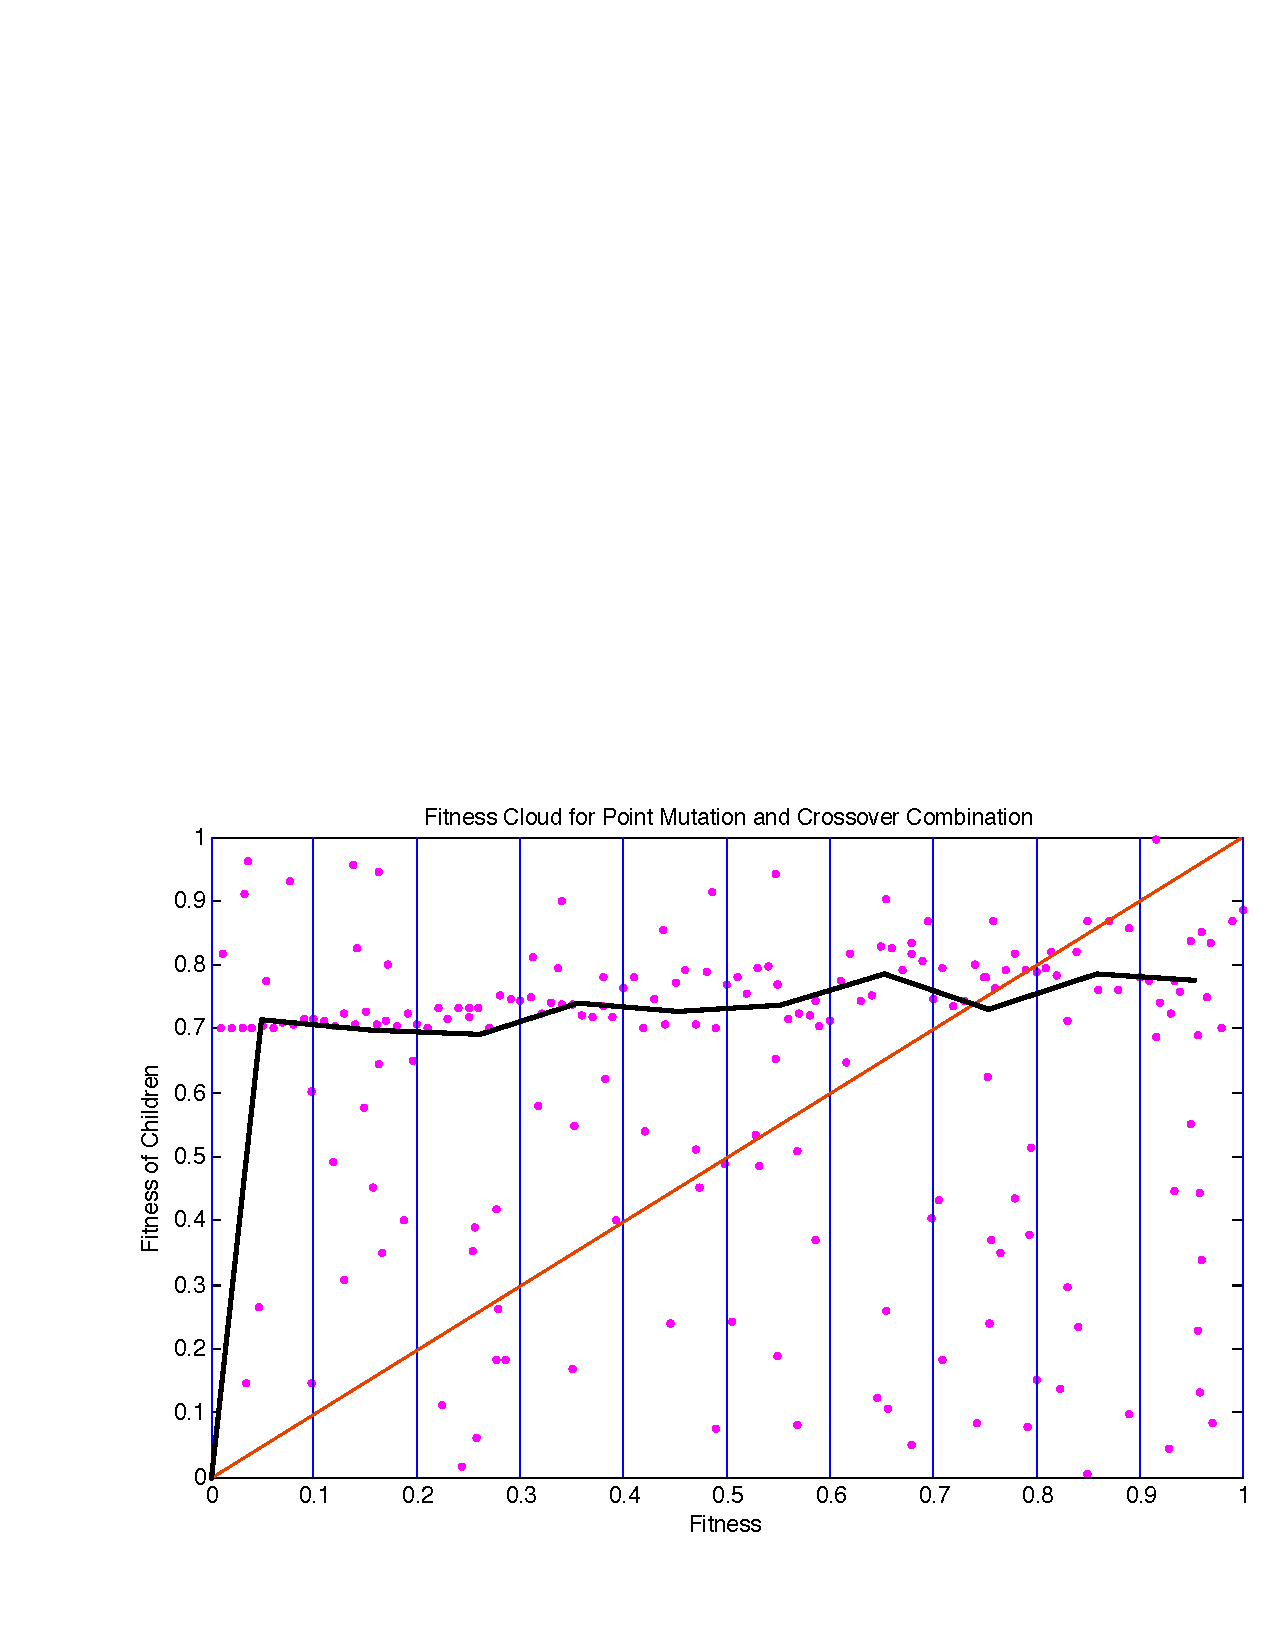
\includegraphics[width=\linewidth]{NSC}
\caption{Calculating the negative slope coefficient}
\end{center}
\end{figure}
\\*
\emph{To decide upon a well-suited intelligent search algorithm for navigating the input space defined by subproblem 1 and to find the best architecture for that algorithm:}

Following for the discussion of intelligent search methods in the Related Literature section, we have chosen to use genetic programming (GP) as the search method for this problem. As Mitchell and Creasey point out, the difficulties in obtaining an optimal solution to a complex search problem are based on several factors, only one of which is the search algorithm itself (2007, p. 1). It is therefore recommended that in order to test only the efficacy of the search, a contrived target should be used. In this problem domain, this means using a target that was generated by a known synthesizer. Mitchell and Creasey suggest randomly generating contrived targets using points uniformly spread out in the input-space (p. 2). If the search algorithm is able to match all of the contrived targets with a good spread in the input space, it is suggested that one can then assume it will be able to match any target (p. 2). This assumes however that a uniformly spread set of points in the input space will map to a large area of the timbre space, which is not necessarily the case. However, more rigorous target testing on non-contrived targets will be carried out within subproblem 5s associated method in case that assumption is invalid.

We will therefore test the search algorithm first on a number of contrived targets with varying degrees of complexity in order to attain an understanding of the limitations of the search algorithm. We will test the algorithm on these targets using different selection and population initialization mechanisms, as the operators themselves will be determined via subproblem 1 and the fitness function via subproblems 4 and 5. A best-of-run average fitness error will be used over all contrived targets for a given selection mechanism (see table 1), and a plot of fitness error vs algorithm complexity (measured as the size of the topology) will be generated for each architecture (see fig. 2). The results obtained will be compared to find the best selection mechanism for the algorithm, and, combined with the results from subproblem 1, will be used to define the optimal architecture.
\begin{table}[h!]
\begin{center}
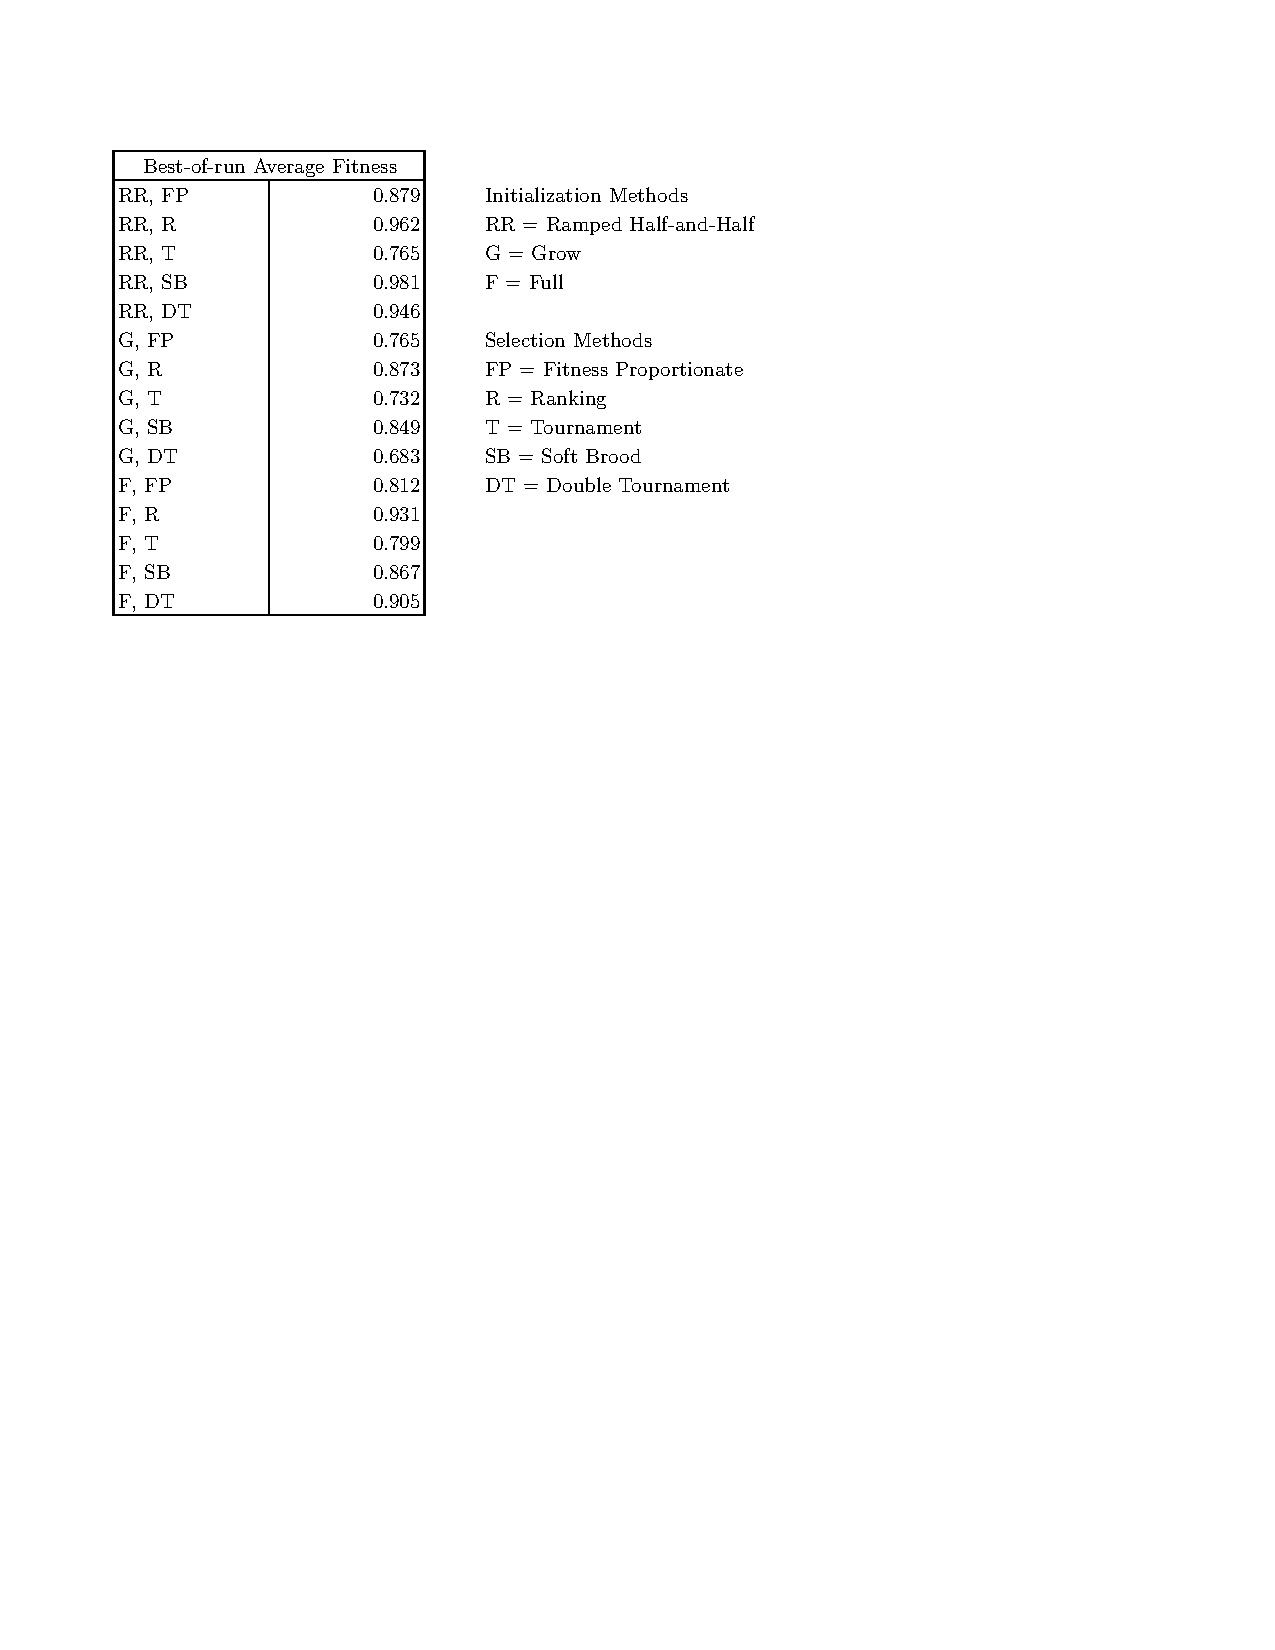
\includegraphics[scale=0.9]{BestOfRunError}
\caption{Average best-of-run fitness}
\end{center}
\end{table}
\begin{figure}[h!]
\begin{center}
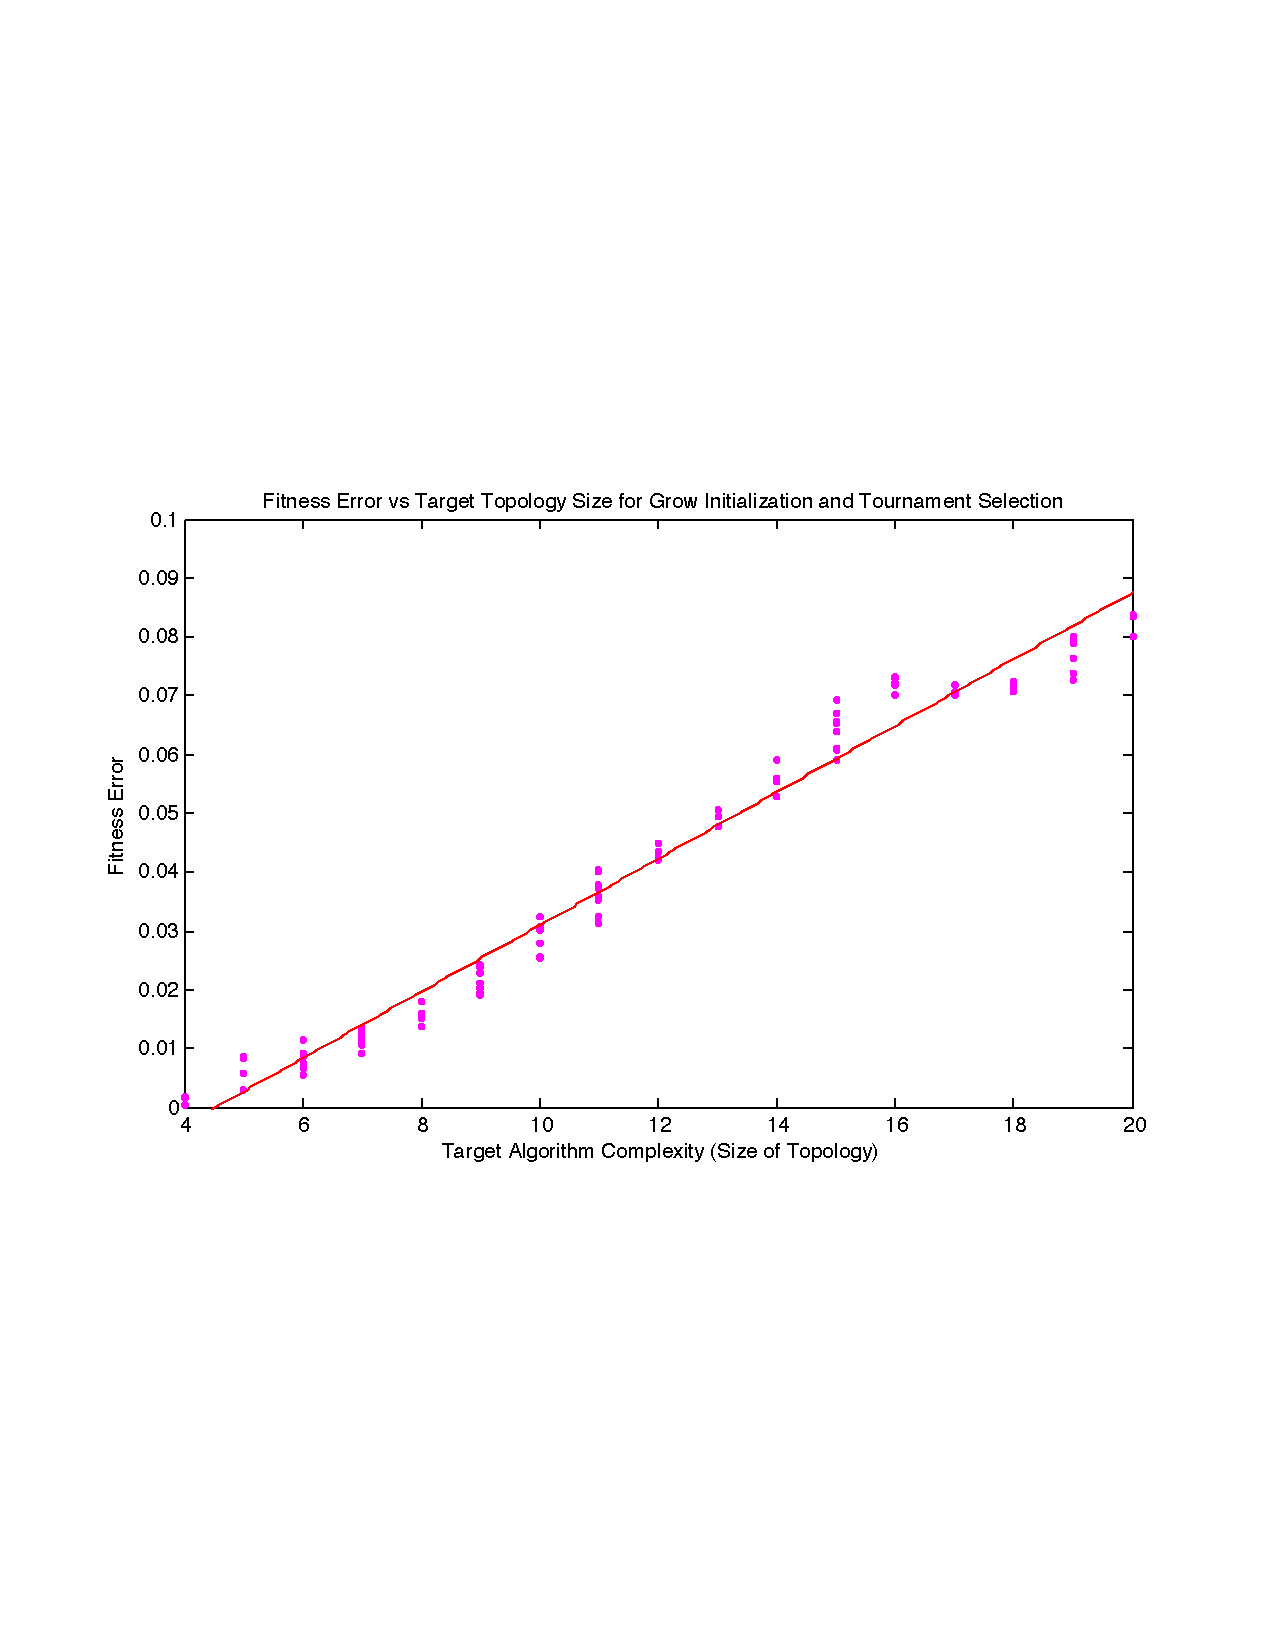
\includegraphics[width=\linewidth]{FEvsAC1}
\caption{Fitness error vs. algorithm complexity}
\end{center}
\end{figure}
\\*
\emph{To find ways of restricting the search space and making the search algorithm more efficient and powerful without omitting optimal solutions:}
In order to improve the efficiency of the search, we will apply a number of methods suggested by the Related Literature including: enforcing strong typing constraints, dynamic maximum tree depth (DMTD) and dynamic resource limited GP (dRLGP) constraints, as well as using increasingly discriminating fitness functions (IFFs). These methods were developed to be used for any problem domain and only discriminate against solutions that are not parsimonious or syntactically valid. They will promote efficiency and low storage requirements as well as controllability of the resulting algorithms due to the propensity to generate low-dimensional parameter sets.

We will also test various degrees to which the parameter space can be discretized and limited and the function set restricted. By placing limitations on the possible parameter and function sets, we hope to restrict the search space even further without excluding optimal solutions. To test the effects of such limitations, we will use the same contrived set of targets from subproblem 2 and plot how error increases as a function of the amount of limitation (see fig. 3). We will also plot how quickly solutions are reached as a function of limitation (see fig. 4). Using the above results, we will be able to obtain an optimal degree of limitation that balances both an increase in efficiency with a decrease in accuracy.
\begin{figure}[h!]
\begin{center}
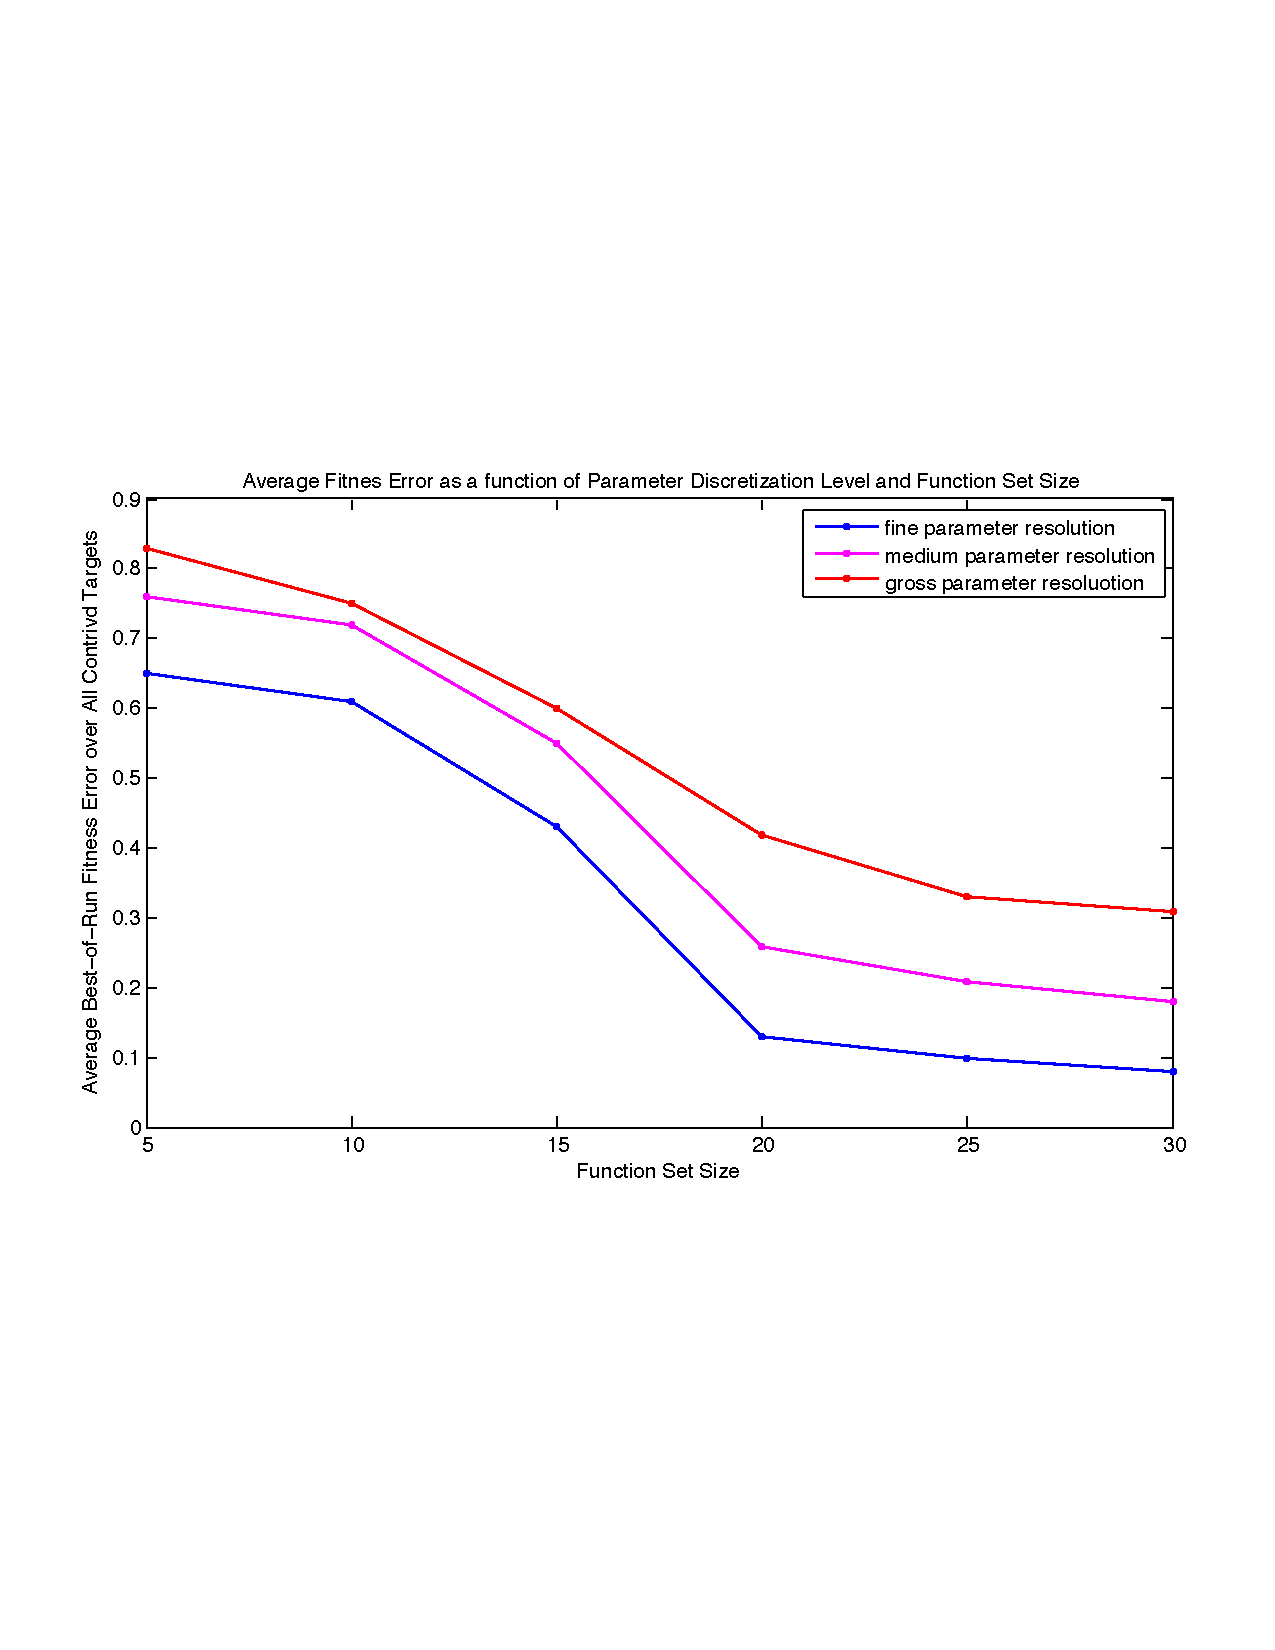
\includegraphics[width=\linewidth]{AFEvsPDL}
\caption{Average fitness error for various building block restrictions}
\end{center}
\end{figure}
\begin{figure}[h!]
\begin{center}
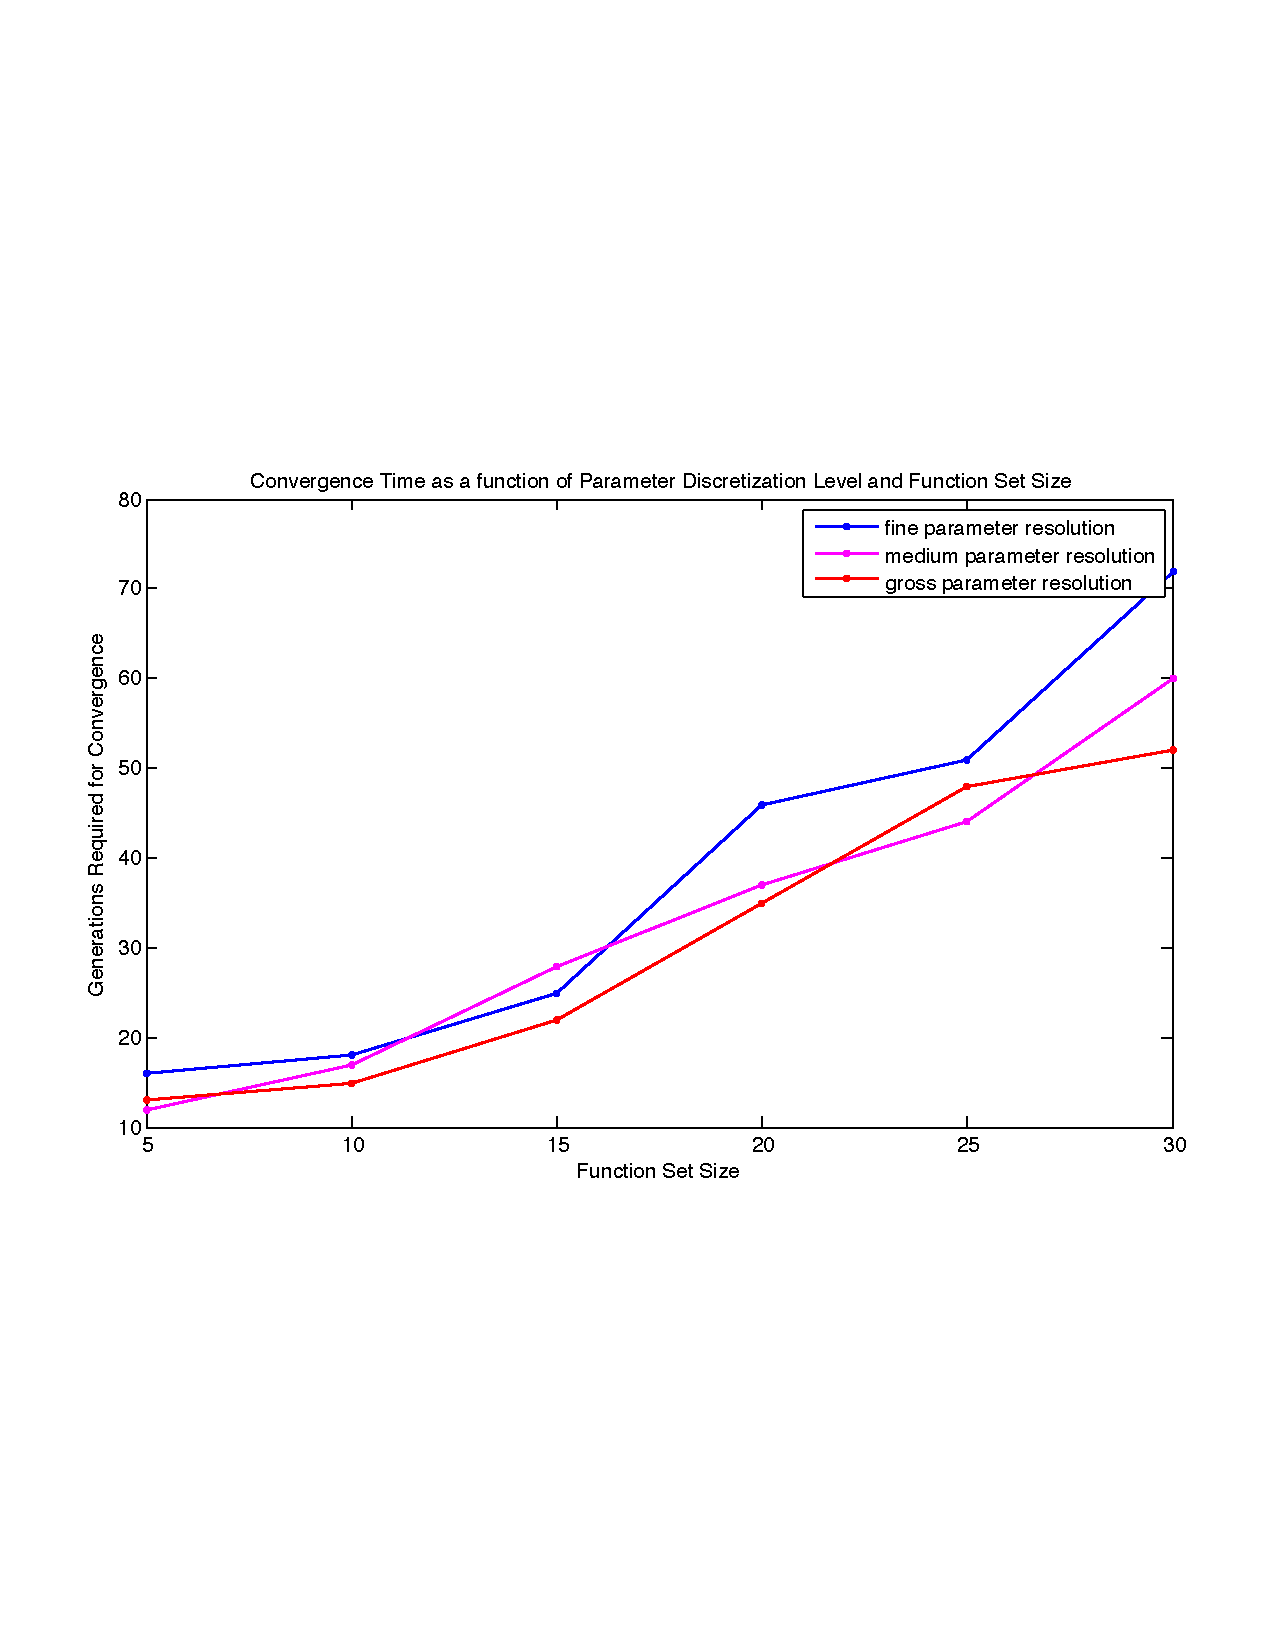
\includegraphics[width=\linewidth]{CTvsPDL}
\caption{Convergence times for various building block restrictions}
\end{center}
\end{figure}
Once such limitations are made explicit, we will compare GP/SA with standard GP in order to determine which is more efficient. These comparisons again will use the contrived set of targets, but will instead only compare the time it takes to reach a specific fitness level for each target. Since the number of algorithms searched per generation differs between GP/SA and standard GP, the number of algorithms searched will be used for a fair comparison (see fig. 5).
\begin{figure}[h!]
\begin{center}
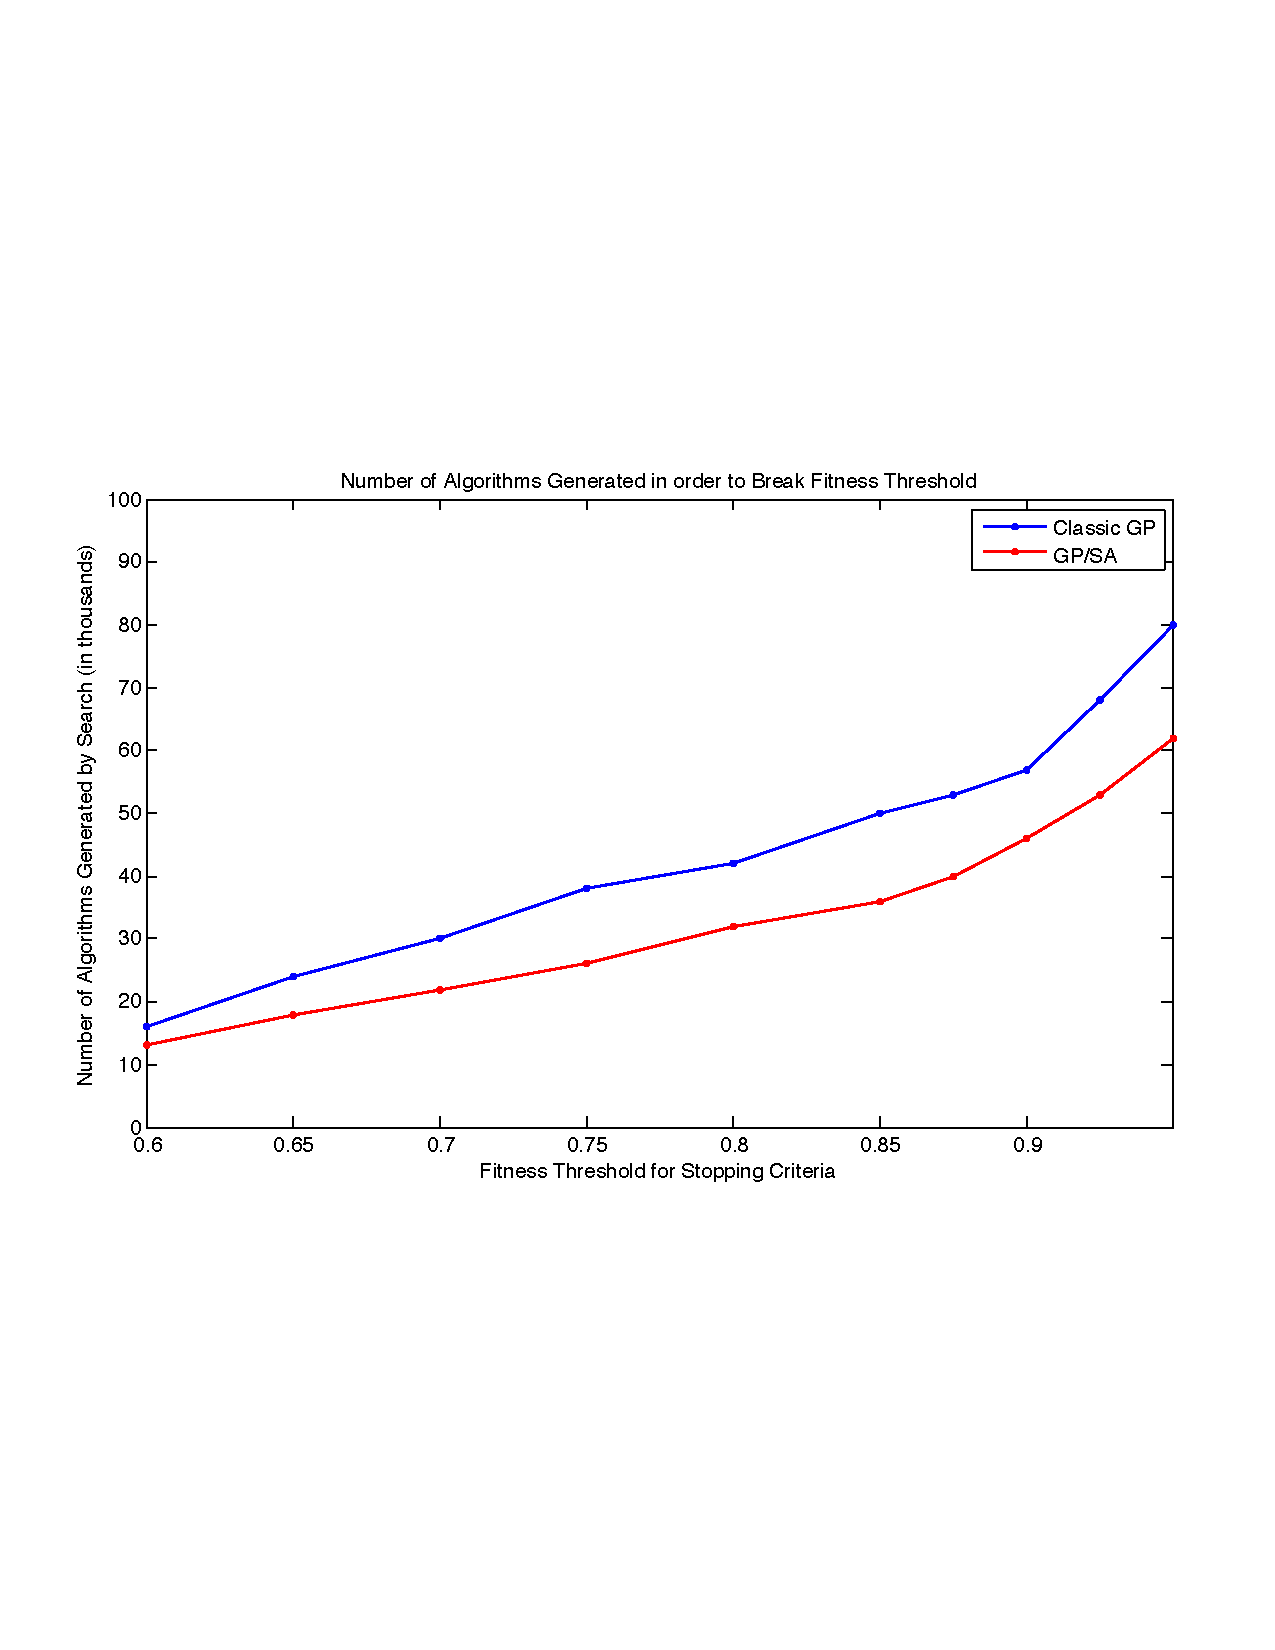
\includegraphics[width=\linewidth]{NAGvsFT}
\caption{Classic GP vs GP/SA efficiency}
\end{center}
\end{figure}
\\*
\emph{To develop an objective timbre space in which distances are semantically meaningful, information regarding the temporal evolution of timbre is retained, and whose elements are invariant to changes in pitch and loudness:}
The design of a semantically valid objective timbre space is paramount to the problem of search. If meaningful timbre similarity measurements cannot be made, then the fitness landscape will be ill-formed and the search will pursue areas of the input space that are not relevant to the problem. 

As previously discussed in the Related Literature, obtaining a ground truth to measure distances against is problematic. While most timbre space evaluation is indirectly performed via classification tasks, due to the cost of doing large scale subjective testing, this evaluation typically assumes that all sounds produced by the same instrument have the same timbre, regardless of playing technique, and so it is not clear that similar evaluation methods will be valid for the `type' of timbre we are interested in. In a recent paper by Pampak, Herrera, and Goto, in referring to timbral studies that use instrument classification as a means of evaluation, the authors note that `instrument class data only allows comparison on the instrument level. Judgements within an instrument class cannot be evaluated directly' (2008, p. 9). 

We understand this issue and will attempt to develop a better way of measuring within instrument timbres throughout our research, but at the very least we will evaluate timbre similarity measures using the standard process of performing a nearest neighbor search within the timbre space in an instrument classification context. This consists of mapping a large database of instrument sound samples into the objective timbre space and measuring how well they cluster by instrument by randomly choosing samples in the space, searching for their nearest neighbor in that space, and recording whether that neighbor was produced by the same instrument. One is then able to compare multiple objective spaces by using the `classification' accuracy found during the experiment. One can extend this experiment by selecting k-nearest neighbors and noting how many of the k neighbors were produced by the same instrument as the test sample.

We will use the above metric to compare a number of timbre objective spaces. As a baseline, we will only use MFCCs. This space will be compared to spaces which include temporal other popular MIR features, features that incorporate early temporal fusion (e.g. Meng's FC coefficients), and features that are learned directly from the data, including those derived from PCA and convolutional Neural Nets.

The results of k-nearest neighbor classification accuracy will be provided for each timbre representation (see table 2).
\begin{table}[h!]
\begin{center}
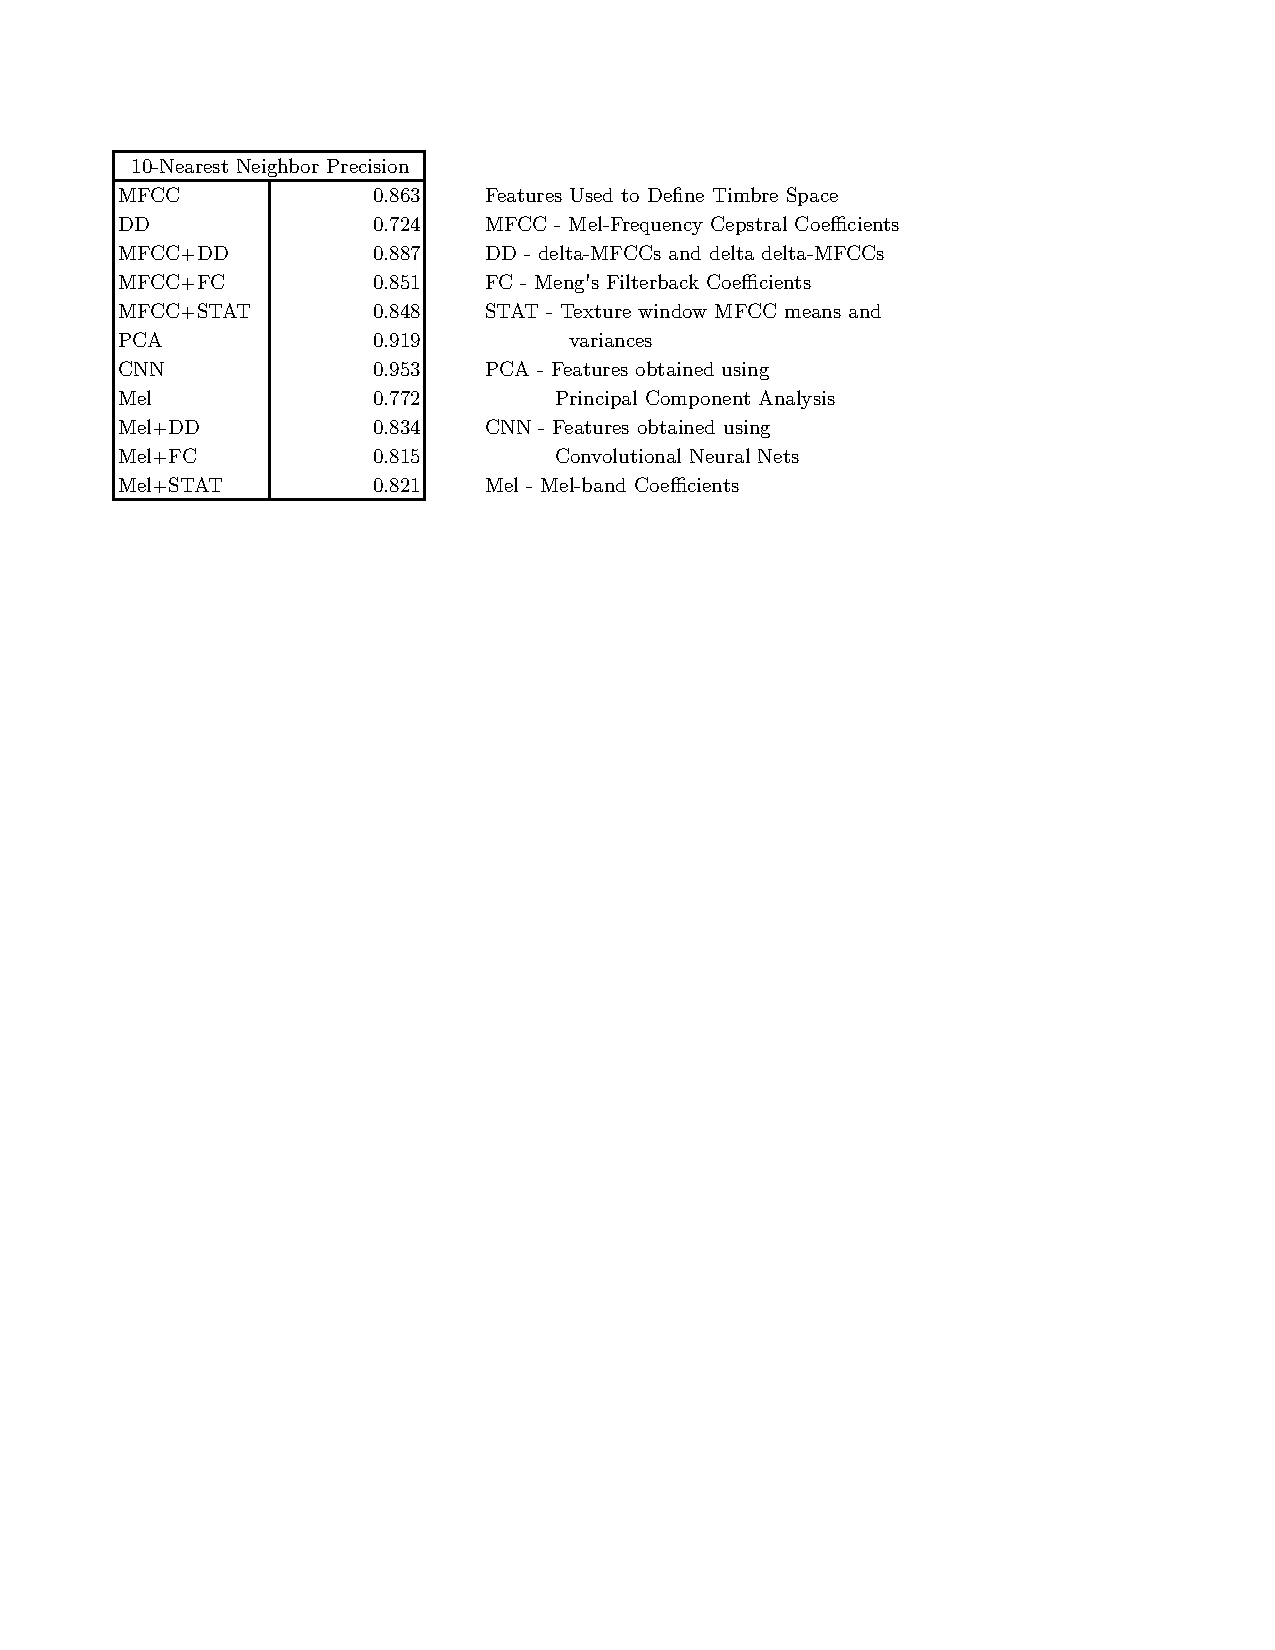
\includegraphics[width=\linewidth]{NN}
\caption{10-nearest neighbor precision}
\end{center}
\end{table}
\\*
\emph{To determine an appropriate similarity metric in the objective timbre space found in subproblem 4 that will be appropriate for comparing time-varying timbral content. This metric will help define an objective landscape over the synthesis algorithm input space whose global maximum (or minimum) will correspond to the desired solution:}

Once an appropriate objective timbre space is defined, one must develop a measure of timbre similarity for time-varying timbres in that space. Timbres that do not vary will only occupy a small region or point in this space. Thus, calculation between two such timbres can simply be performed using Euclidean distance as the space will be developed for this distance to be semantically meaningful. However, once a sound contains timbral variation, tracing out a trajectory in timbre space, it is not trivial to determine how similar other time-varying timbres are to it. Simply lining up points in these trajectories and calculating a summed Euclidean distance of pairs will not be invariant to slight time shifts or warpings. It is for this reason that Jehan uses DTW when calculating similarity over sound segments (2005). The only difference is the time scale on which similarity is being computed.

We therefore seek a local timbre similarity metric that is invariant to time shifts, warpings, and other temporal distortions. We will test relevant models (e.g. HMM, DTW) using a number of temporally distorted sample files. The distortions applied will include global time scaling and time shifting, local time warping, random sample deletion, and random extension of stable timbral content. We will measure how invariant each model is to these temporal distortions by considering a nonzero distance between the original sample and one of its distorted versions as an error. We will measure these errors given a number of different sample files and average over each distortion. This will be performed over varying levels of severity for each specific distortion (see fig. 6).
\begin{figure}[h!]
\begin{center}
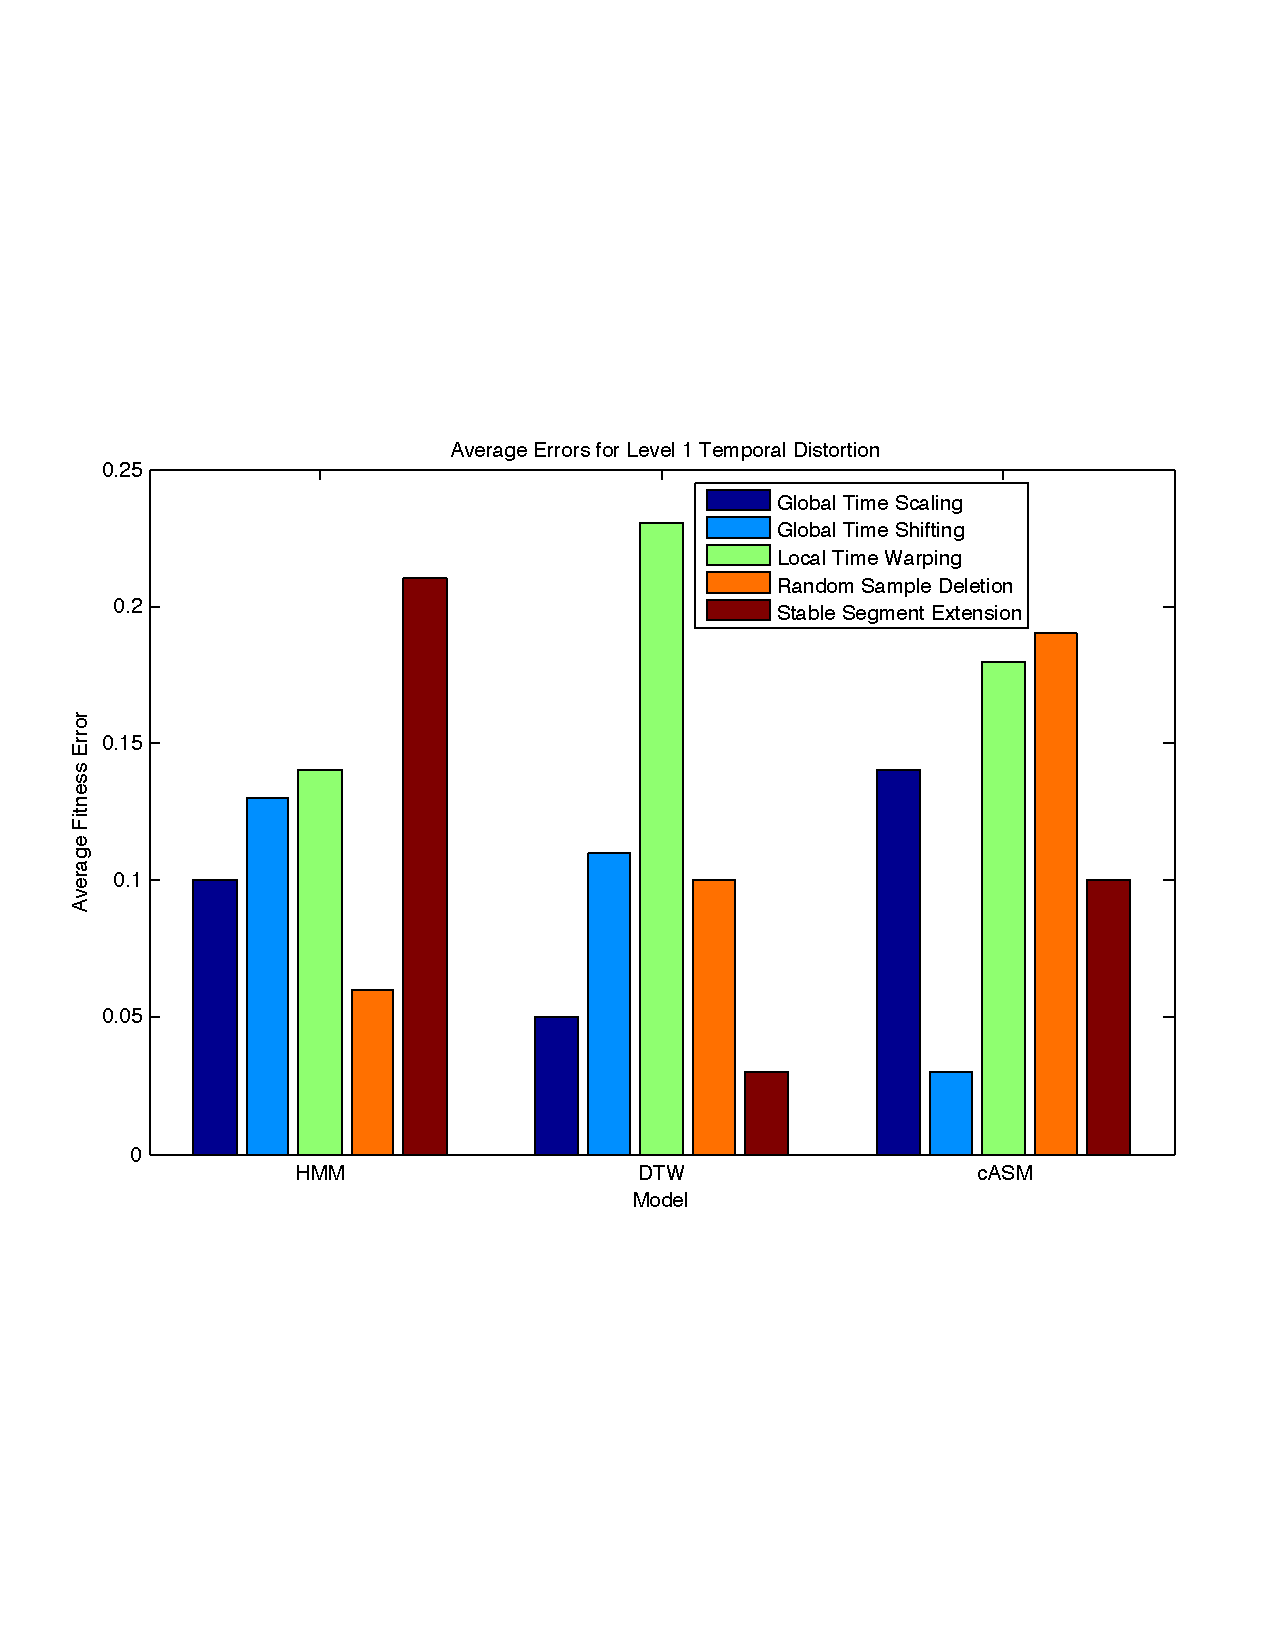
\includegraphics[width=\linewidth]{AEvsMOD}
\caption{Average model error for level 1 (mild) distortions}
\end{center}
\end{figure}
\\*
\emph{To combine the solutions of subproblems 1-5 into a system implementation capable of automatically generating synthesis algorithms that not only match the target input, but that also exhibit attractive properties for any synthesis algorithm:}
I will use all of the results obtained from the previously mentioned methods to influence implementation decisions for the construction of a system in C++ that is able to automatically generate patches in Max that accurately model the timbre of a target sound.

It will be necessary to test this system on a number of real-world sounds in order to gauge its ability to generalize to sounds that are not contrived. As Riionheimo and Valimaki note, `the quality of resynthesis of real recordings is more difficult to measure as there are no known correct parameter values' nor synthesis topologies (2003, p. 13). In genetic programming research where a known target algorithm does not exist, the performance of the system is usually measured using the fitness level at which the system converges and how long it takes to converge to that level. Thus, using a number of different test recordings, we will generate the following statistics: mean fitness per generation, max fitness per generation, min fitness per generation, and best fitness over a run with the corresponding generation number at which that is found. These statistics will then be used to determine the mean and variance of best run individuals given no time constraints (i.e. allowing search to converge), as well as best run individuals produced given a number of different time constraints (e.g. at multiples of 10 generations) (see table 3).
\begin{table}[h!]
\begin{center}
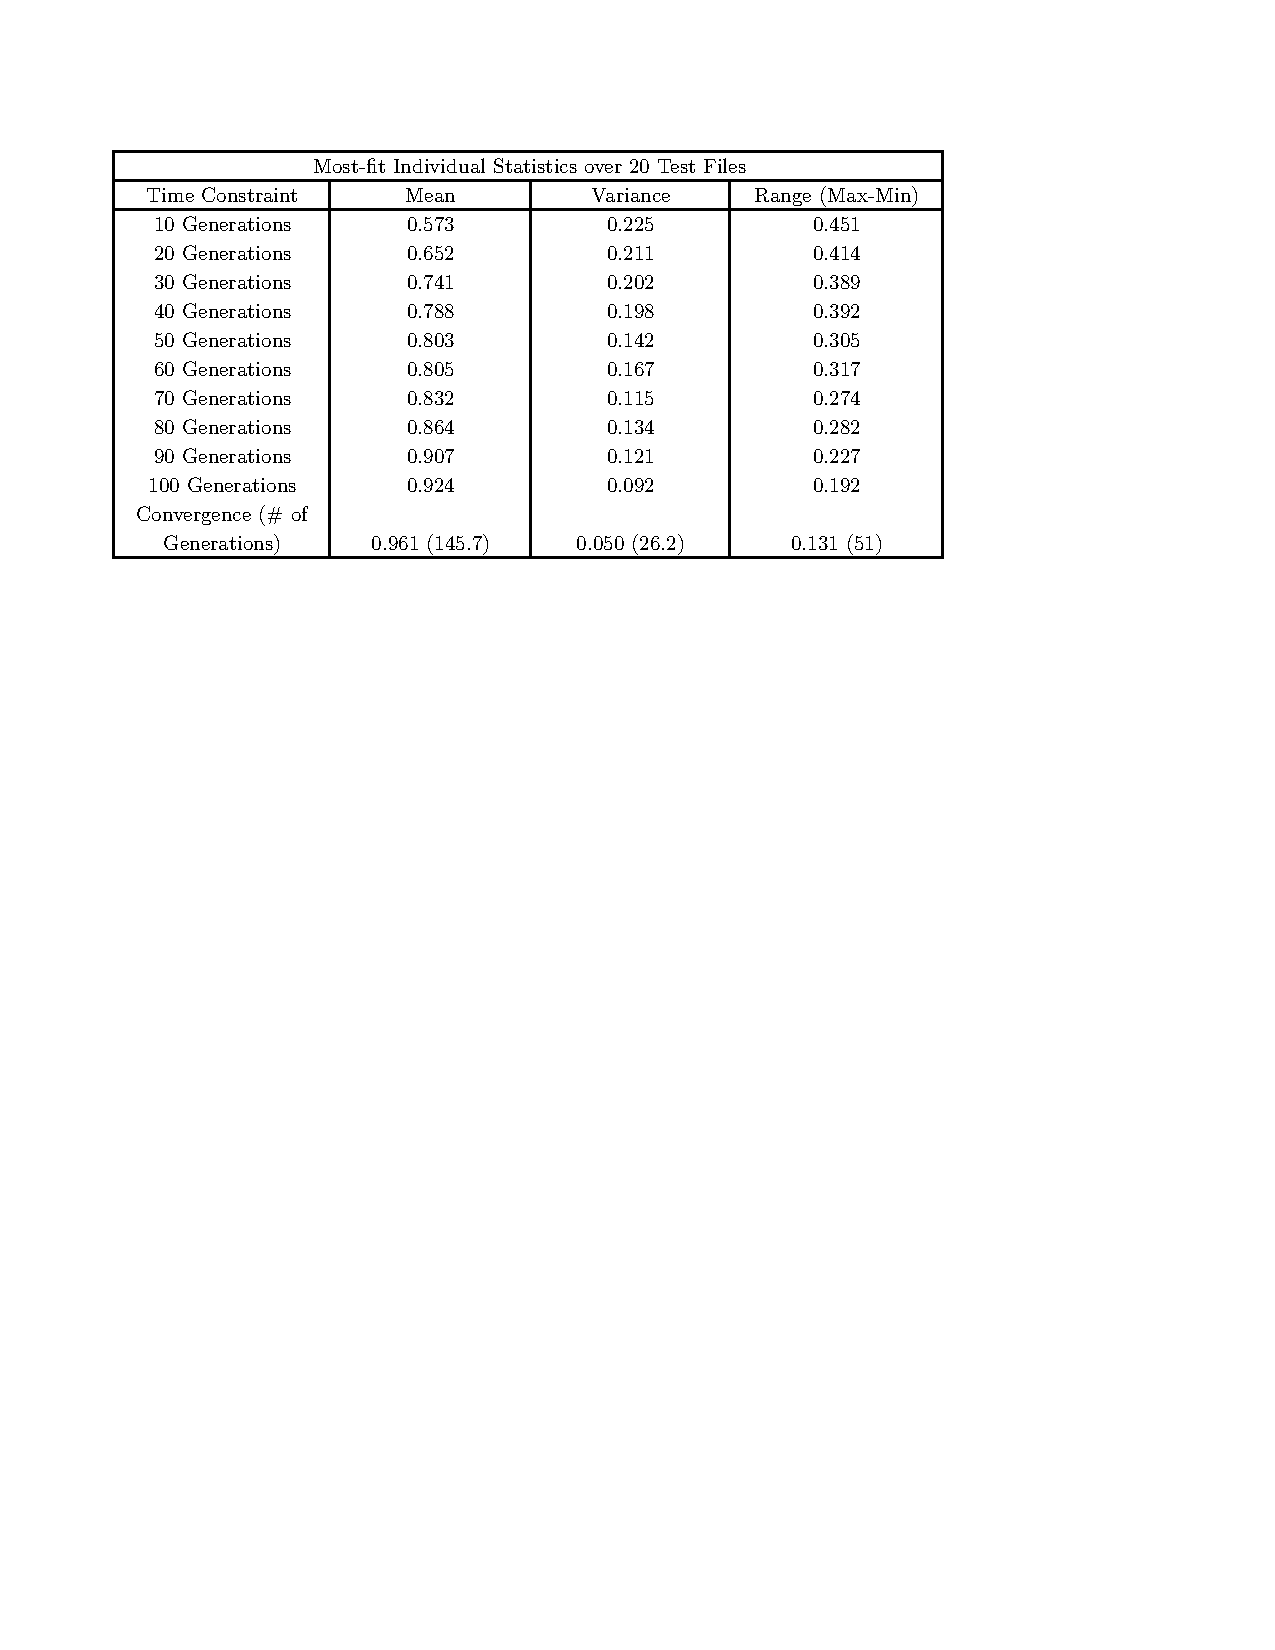
\includegraphics[width=\linewidth]{BestOfRun}
\caption{Best-of-run statistics over 20 test targets}
\end{center}
\end{table}

\end{flushleft}
\newpage
\nocite{*}	% This says to cite all refs in the bib file
\bibliographystyle{apacite}	% apa style
\bibliography{mybib}		% name of bib file 

\end{document}